\documentclass[twoside]{book}

% Packages required by doxygen
\usepackage{fixltx2e}
\usepackage{calc}
\usepackage{doxygen}
\usepackage[export]{adjustbox} % also loads graphicx
\usepackage{graphicx}
\usepackage[utf8]{inputenc}
\usepackage{makeidx}
\usepackage{multicol}
\usepackage{multirow}
\PassOptionsToPackage{warn}{textcomp}
\usepackage{textcomp}
\usepackage[nointegrals]{wasysym}
\usepackage[table]{xcolor}

% Font selection
\usepackage[T1]{fontenc}
\usepackage[scaled=.90]{helvet}
\usepackage{courier}
\usepackage{amssymb}
\usepackage{sectsty}
\renewcommand{\familydefault}{\sfdefault}
\allsectionsfont{%
  \fontseries{bc}\selectfont%
  \color{darkgray}%
}
\renewcommand{\DoxyLabelFont}{%
  \fontseries{bc}\selectfont%
  \color{darkgray}%
}
\newcommand{\+}{\discretionary{\mbox{\scriptsize$\hookleftarrow$}}{}{}}

% Page & text layout
\usepackage{geometry}
\geometry{%
  a4paper,%
  top=2.5cm,%
  bottom=2.5cm,%
  left=2.5cm,%
  right=2.5cm%
}
\tolerance=750
\hfuzz=15pt
\hbadness=750
\setlength{\emergencystretch}{15pt}
\setlength{\parindent}{0cm}
\setlength{\parskip}{3ex plus 2ex minus 2ex}
\makeatletter
\renewcommand{\paragraph}{%
  \@startsection{paragraph}{4}{0ex}{-1.0ex}{1.0ex}{%
    \normalfont\normalsize\bfseries\SS@parafont%
  }%
}
\renewcommand{\subparagraph}{%
  \@startsection{subparagraph}{5}{0ex}{-1.0ex}{1.0ex}{%
    \normalfont\normalsize\bfseries\SS@subparafont%
  }%
}
\makeatother

% Headers & footers
\usepackage{fancyhdr}
\pagestyle{fancyplain}
\fancyhead[LE]{\fancyplain{}{\bfseries\thepage}}
\fancyhead[CE]{\fancyplain{}{}}
\fancyhead[RE]{\fancyplain{}{\bfseries\leftmark}}
\fancyhead[LO]{\fancyplain{}{\bfseries\rightmark}}
\fancyhead[CO]{\fancyplain{}{}}
\fancyhead[RO]{\fancyplain{}{\bfseries\thepage}}
\fancyfoot[LE]{\fancyplain{}{}}
\fancyfoot[CE]{\fancyplain{}{}}
\fancyfoot[RE]{\fancyplain{}{\bfseries\scriptsize Generated by Doxygen }}
\fancyfoot[LO]{\fancyplain{}{\bfseries\scriptsize Generated by Doxygen }}
\fancyfoot[CO]{\fancyplain{}{}}
\fancyfoot[RO]{\fancyplain{}{}}
\renewcommand{\footrulewidth}{0.4pt}
\renewcommand{\chaptermark}[1]{%
  \markboth{#1}{}%
}
\renewcommand{\sectionmark}[1]{%
  \markright{\thesection\ #1}%
}

% Indices & bibliography
\usepackage{natbib}
\usepackage[titles]{tocloft}
\setcounter{tocdepth}{3}
\setcounter{secnumdepth}{5}
\makeindex

% Hyperlinks (required, but should be loaded last)
\usepackage{ifpdf}
\ifpdf
  \usepackage[pdftex,pagebackref=true]{hyperref}
\else
  \usepackage[ps2pdf,pagebackref=true]{hyperref}
\fi
\hypersetup{%
  colorlinks=true,%
  linkcolor=blue,%
  citecolor=blue,%
  unicode%
}

% Custom commands
\newcommand{\clearemptydoublepage}{%
  \newpage{\pagestyle{empty}\cleardoublepage}%
}

\usepackage{caption}
\captionsetup{labelsep=space,justification=centering,font={bf},singlelinecheck=off,skip=4pt,position=top}

%===== C O N T E N T S =====

\begin{document}

% Titlepage & ToC
\hypersetup{pageanchor=false,
             bookmarksnumbered=true,
             pdfencoding=unicode
            }
\pagenumbering{alph}
\begin{titlepage}
\vspace*{7cm}
\begin{center}%
{\Large Optim\+\_\+\+V\+S\+T\+R\+AP }\\
\vspace*{1cm}
{\large Generated by Doxygen 1.8.13}\\
\end{center}
\end{titlepage}
\clearemptydoublepage
\pagenumbering{roman}
\tableofcontents
\clearemptydoublepage
\pagenumbering{arabic}
\hypersetup{pageanchor=true}

%--- Begin generated contents ---
\chapter{Hierarchical Index}
\section{Class Hierarchy}
This inheritance list is sorted roughly, but not completely, alphabetically\+:\begin{DoxyCompactList}
\item \contentsline{section}{abstract\+\_\+controller}{\pageref{classabstract__controller}}{}
\begin{DoxyCompactList}
\item \contentsline{section}{desired\+\_\+trajectory\+\_\+controller}{\pageref{classdesired__trajectory__controller}}{}
\item \contentsline{section}{equation\+\_\+solving\+\_\+controller}{\pageref{classequation__solving__controller}}{}
\item \contentsline{section}{gradient\+\_\+calculator}{\pageref{classgradient__calculator}}{}
\item \contentsline{section}{input}{\pageref{classinput}}{}
\item \contentsline{section}{objective\+\_\+calculator}{\pageref{classobjective__calculator}}{}
\item \contentsline{section}{optim\+\_\+controller}{\pageref{classoptim__controller}}{}
\item \contentsline{section}{output\+\_\+control\+\_\+update}{\pageref{classoutput__control__update}}{}
\item \contentsline{section}{output\+\_\+diagnostics}{\pageref{classoutput__diagnostics}}{}
\item \contentsline{section}{pdf\+\_\+controller}{\pageref{classpdf__controller}}{}
\item \contentsline{section}{stepdirection\+\_\+controller}{\pageref{classstepdirection__controller}}{}
\item \contentsline{section}{stepsize\+\_\+controller}{\pageref{classstepsize__controller}}{}
\end{DoxyCompactList}
\item \contentsline{section}{mesh.\+Cell}{\pageref{classmesh_1_1Cell}}{}
\item \contentsline{section}{control\+\_\+field\+\_\+class.\+Control\+\_\+field}{\pageref{classcontrol__field__class_1_1Control__field}}{}
\item \contentsline{section}{coordinate\+\_\+phase\+\_\+space\+\_\+time}{\pageref{classcoordinate__phase__space__time}}{}
\item \contentsline{section}{data\+\_\+provider}{\pageref{classdata__provider}}{}
\item \contentsline{section}{std\+:\+:hash$<$ coordinate\+\_\+phase\+\_\+space\+\_\+time $>$}{\pageref{structstd_1_1hash_3_01coordinate__phase__space__time_01_4}}{}
\item \contentsline{section}{mesh.\+Mesh}{\pageref{classmesh_1_1Mesh}}{}
\item \contentsline{section}{mesh.\+Node}{\pageref{classmesh_1_1Node}}{}
\item \contentsline{section}{particle}{\pageref{classparticle}}{}
\item Test\+Case\begin{DoxyCompactList}
\item \contentsline{section}{mesh.\+Cell\+Test}{\pageref{classmesh_1_1CellTest}}{}
\item \contentsline{section}{mesh.\+Mesh\+Test}{\pageref{classmesh_1_1MeshTest}}{}
\end{DoxyCompactList}
\item Fancy\+Arrow\+Patch\begin{DoxyCompactList}
\item \contentsline{section}{control\+\_\+field\+\_\+class.\+Arrow3D}{\pageref{classcontrol__field__class_1_1Arrow3D}}{}
\end{DoxyCompactList}
\end{DoxyCompactList}

\chapter{Class Index}
\section{Class List}
Here are the classes, structs, unions and interfaces with brief descriptions\+:\begin{DoxyCompactList}
\item\contentsline{section}{\hyperlink{classabstract__controller}{abstract\+\_\+controller} }{\pageref{classabstract__controller}}{}
\item\contentsline{section}{\hyperlink{classcontrol__field__class_1_1Arrow3D}{control\+\_\+field\+\_\+class.\+Arrow3D} }{\pageref{classcontrol__field__class_1_1Arrow3D}}{}
\item\contentsline{section}{\hyperlink{classmesh_1_1Cell}{mesh.\+Cell} }{\pageref{classmesh_1_1Cell}}{}
\item\contentsline{section}{\hyperlink{classmesh_1_1CellTest}{mesh.\+Cell\+Test} }{\pageref{classmesh_1_1CellTest}}{}
\item\contentsline{section}{\hyperlink{classcontrol__field__class_1_1Control__field}{control\+\_\+field\+\_\+class.\+Control\+\_\+field} }{\pageref{classcontrol__field__class_1_1Control__field}}{}
\item\contentsline{section}{\hyperlink{classcoordinate__phase__space__time}{coordinate\+\_\+phase\+\_\+space\+\_\+time} }{\pageref{classcoordinate__phase__space__time}}{}
\item\contentsline{section}{\hyperlink{classdata__provider}{data\+\_\+provider} }{\pageref{classdata__provider}}{}
\item\contentsline{section}{\hyperlink{classdesired__trajectory__controller}{desired\+\_\+trajectory\+\_\+controller} }{\pageref{classdesired__trajectory__controller}}{}
\item\contentsline{section}{\hyperlink{classequation__solving__controller}{equation\+\_\+solving\+\_\+controller} }{\pageref{classequation__solving__controller}}{}
\item\contentsline{section}{\hyperlink{classgradient__calculator}{gradient\+\_\+calculator} }{\pageref{classgradient__calculator}}{}
\item\contentsline{section}{\hyperlink{structstd_1_1hash_3_01coordinate__phase__space__time_01_4}{std\+::hash$<$ coordinate\+\_\+phase\+\_\+space\+\_\+time $>$} }{\pageref{structstd_1_1hash_3_01coordinate__phase__space__time_01_4}}{}
\item\contentsline{section}{\hyperlink{classinput}{input} }{\pageref{classinput}}{}
\item\contentsline{section}{\hyperlink{classmesh_1_1Mesh}{mesh.\+Mesh} }{\pageref{classmesh_1_1Mesh}}{}
\item\contentsline{section}{\hyperlink{classmesh_1_1MeshTest}{mesh.\+Mesh\+Test} }{\pageref{classmesh_1_1MeshTest}}{}
\item\contentsline{section}{\hyperlink{classmesh_1_1Node}{mesh.\+Node} }{\pageref{classmesh_1_1Node}}{}
\item\contentsline{section}{\hyperlink{classobjective__calculator}{objective\+\_\+calculator} }{\pageref{classobjective__calculator}}{}
\item\contentsline{section}{\hyperlink{classoptim__controller}{optim\+\_\+controller} }{\pageref{classoptim__controller}}{}
\item\contentsline{section}{\hyperlink{classoutput__control__update}{output\+\_\+control\+\_\+update} \\*Offers functions to write the update of the control in a file that is readable by the solver for forward and backward equation }{\pageref{classoutput__control__update}}{}
\item\contentsline{section}{\hyperlink{classoutput__diagnostics}{output\+\_\+diagnostics} }{\pageref{classoutput__diagnostics}}{}
\item\contentsline{section}{\hyperlink{classparticle}{particle} }{\pageref{classparticle}}{}
\item\contentsline{section}{\hyperlink{classpdf__controller}{pdf\+\_\+controller} }{\pageref{classpdf__controller}}{}
\item\contentsline{section}{\hyperlink{classstepdirection__controller}{stepdirection\+\_\+controller} }{\pageref{classstepdirection__controller}}{}
\item\contentsline{section}{\hyperlink{classstepsize__controller}{stepsize\+\_\+controller} }{\pageref{classstepsize__controller}}{}
\end{DoxyCompactList}

\chapter{Class Documentation}
\hypertarget{classabstract__controller}{}\section{abstract\+\_\+controller Class Reference}
\label{classabstract__controller}\index{abstract\+\_\+controller@{abstract\+\_\+controller}}


Inheritance diagram for abstract\+\_\+controller\+:\nopagebreak
\begin{figure}[H]
\begin{center}
\leavevmode
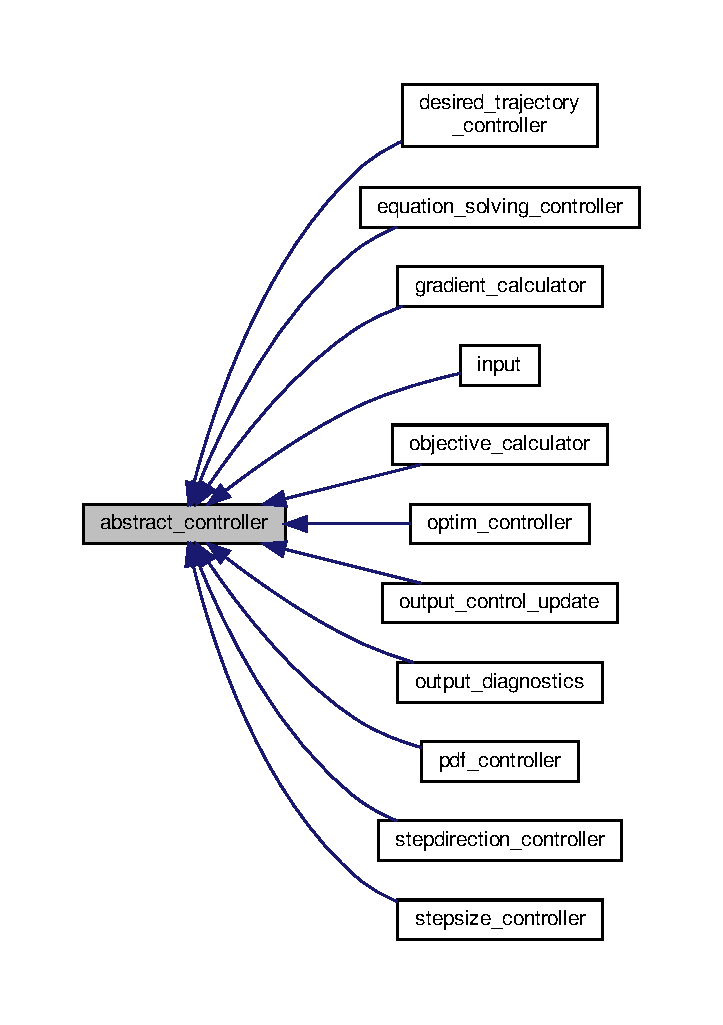
\includegraphics[width=347pt]{classabstract__controller__inherit__graph}
\end{center}
\end{figure}
\subsection*{Public Member Functions}
\begin{DoxyCompactItemize}
\item 
\mbox{\Hypertarget{classabstract__controller_ae4a15450620978e51c578666d359349c}\label{classabstract__controller_ae4a15450620978e51c578666d359349c}} 
\hyperlink{classdata__provider}{data\+\_\+provider} {\bfseries get\+Data\+\_\+provider\+\_\+optim} () const
\item 
\mbox{\Hypertarget{classabstract__controller_a35988272a58784db06c9d1e48f0a3292}\label{classabstract__controller_a35988272a58784db06c9d1e48f0a3292}} 
void {\bfseries set\+Data\+\_\+provider\+\_\+optim} (const \hyperlink{classdata__provider}{data\+\_\+provider} \&value)
\end{DoxyCompactItemize}


The documentation for this class was generated from the following files\+:\begin{DoxyCompactItemize}
\item 
/home/jan/\+Promotion\+\_\+linux\+P\+C/\+Optim\+\_\+\+V\+S\+T\+R\+A\+P/src/controller/abstract\+\_\+controller.\+h\item 
/home/jan/\+Promotion\+\_\+linux\+P\+C/\+Optim\+\_\+\+V\+S\+T\+R\+A\+P/src/controller/abstract\+\_\+controller.\+cpp\end{DoxyCompactItemize}

\hypertarget{classcontrol__field__class_1_1Arrow3D}{}\section{control\+\_\+field\+\_\+class.\+Arrow3D Class Reference}
\label{classcontrol__field__class_1_1Arrow3D}\index{control\+\_\+field\+\_\+class.\+Arrow3D@{control\+\_\+field\+\_\+class.\+Arrow3D}}


Inheritance diagram for control\+\_\+field\+\_\+class.\+Arrow3D\+:\nopagebreak
\begin{figure}[H]
\begin{center}
\leavevmode
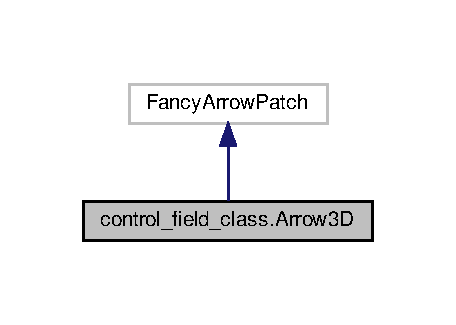
\includegraphics[width=219pt]{classcontrol__field__class_1_1Arrow3D__inherit__graph}
\end{center}
\end{figure}


Collaboration diagram for control\+\_\+field\+\_\+class.\+Arrow3D\+:\nopagebreak
\begin{figure}[H]
\begin{center}
\leavevmode
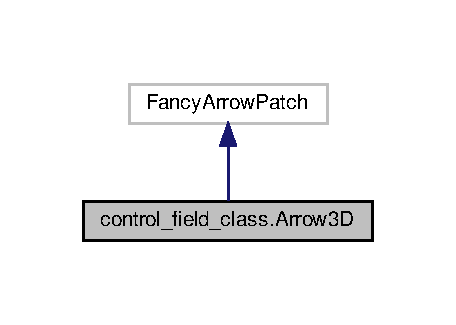
\includegraphics[width=219pt]{classcontrol__field__class_1_1Arrow3D__coll__graph}
\end{center}
\end{figure}
\subsection*{Public Member Functions}
\begin{DoxyCompactItemize}
\item 
\mbox{\Hypertarget{classcontrol__field__class_1_1Arrow3D_af98fc15e10ed35ec3cfaba0db76e7339}\label{classcontrol__field__class_1_1Arrow3D_af98fc15e10ed35ec3cfaba0db76e7339}} 
def {\bfseries \+\_\+\+\_\+init\+\_\+\+\_\+} (self, xs, ys, zs, args, kwargs)
\item 
\mbox{\Hypertarget{classcontrol__field__class_1_1Arrow3D_a467839333d88e604fef2abca849b9311}\label{classcontrol__field__class_1_1Arrow3D_a467839333d88e604fef2abca849b9311}} 
def {\bfseries draw} (self, renderer)
\end{DoxyCompactItemize}


The documentation for this class was generated from the following file\+:\begin{DoxyCompactItemize}
\item 
/home/jan/\+Promotion\+\_\+linux\+P\+C/\+Optim\+\_\+\+V\+S\+T\+R\+A\+P/optim-\/vstrap-\/toolset/toolset/control\+\_\+field\+\_\+class.\+py\end{DoxyCompactItemize}

\hypertarget{classmesh_1_1Cell}{}\section{mesh.\+Cell Class Reference}
\label{classmesh_1_1Cell}\index{mesh.\+Cell@{mesh.\+Cell}}
\subsection*{Public Member Functions}
\begin{DoxyCompactItemize}
\item 
\mbox{\Hypertarget{classmesh_1_1Cell_a6c61268b0162ea1a3323c1def2bc505a}\label{classmesh_1_1Cell_a6c61268b0162ea1a3323c1def2bc505a}} 
def {\bfseries \+\_\+\+\_\+init\+\_\+\+\_\+} (self)
\item 
\mbox{\Hypertarget{classmesh_1_1Cell_abb04a423222f1f5ccbf1700249f75f90}\label{classmesh_1_1Cell_abb04a423222f1f5ccbf1700249f75f90}} 
def {\bfseries set\+\_\+nodes} (self, nodes)
\item 
\mbox{\Hypertarget{classmesh_1_1Cell_ab4c0e290a8b94f1bf46507c3fb56a0ea}\label{classmesh_1_1Cell_ab4c0e290a8b94f1bf46507c3fb56a0ea}} 
def {\bfseries calc\+\_\+volume} (self, nodes)
\item 
\mbox{\Hypertarget{classmesh_1_1Cell_afcaf55fc2ee39266624ecb7439a8ce6a}\label{classmesh_1_1Cell_afcaf55fc2ee39266624ecb7439a8ce6a}} 
def {\bfseries calc\+\_\+barycenter} (self, nodes)
\end{DoxyCompactItemize}
\subsection*{Public Attributes}
\begin{DoxyCompactItemize}
\item 
\mbox{\Hypertarget{classmesh_1_1Cell_a0c625c512240ebff7d8426b17300f1c1}\label{classmesh_1_1Cell_a0c625c512240ebff7d8426b17300f1c1}} 
{\bfseries id}
\item 
\mbox{\Hypertarget{classmesh_1_1Cell_a205e213f2e3f1b1290787f93e4f0f5c0}\label{classmesh_1_1Cell_a205e213f2e3f1b1290787f93e4f0f5c0}} 
{\bfseries nodes\+\_\+ids}
\item 
\mbox{\Hypertarget{classmesh_1_1Cell_a030dce3c25e3f14db97bebc69a75101c}\label{classmesh_1_1Cell_a030dce3c25e3f14db97bebc69a75101c}} 
{\bfseries value}
\item 
\mbox{\Hypertarget{classmesh_1_1Cell_ad7fc1b9f8868b77bbb387b9207004e93}\label{classmesh_1_1Cell_ad7fc1b9f8868b77bbb387b9207004e93}} 
{\bfseries volume}
\item 
\mbox{\Hypertarget{classmesh_1_1Cell_a19509c56b82d6c920fd15b83f5eb6202}\label{classmesh_1_1Cell_a19509c56b82d6c920fd15b83f5eb6202}} 
{\bfseries type}
\item 
\mbox{\Hypertarget{classmesh_1_1Cell_ad890a38b19a74dc227f535756f0583b3}\label{classmesh_1_1Cell_ad890a38b19a74dc227f535756f0583b3}} 
{\bfseries barycenter}
\end{DoxyCompactItemize}


The documentation for this class was generated from the following file\+:\begin{DoxyCompactItemize}
\item 
/home/jan/\+Promotion\+\_\+linux\+P\+C/\+Optim\+\_\+\+V\+S\+T\+R\+A\+P/optim-\/vstrap-\/toolset/toolset/mesh.\+py\end{DoxyCompactItemize}

\hypertarget{classmesh_1_1CellTest}{}\section{mesh.\+Cell\+Test Class Reference}
\label{classmesh_1_1CellTest}\index{mesh.\+Cell\+Test@{mesh.\+Cell\+Test}}


Inheritance diagram for mesh.\+Cell\+Test\+:\nopagebreak
\begin{figure}[H]
\begin{center}
\leavevmode
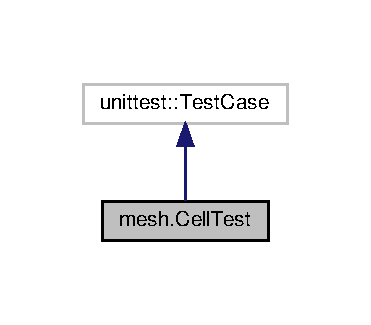
\includegraphics[width=178pt]{classmesh_1_1CellTest__inherit__graph}
\end{center}
\end{figure}


Collaboration diagram for mesh.\+Cell\+Test\+:\nopagebreak
\begin{figure}[H]
\begin{center}
\leavevmode
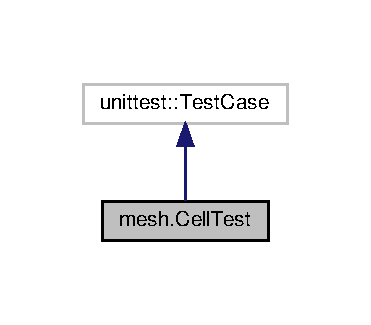
\includegraphics[width=178pt]{classmesh_1_1CellTest__coll__graph}
\end{center}
\end{figure}
\subsection*{Public Member Functions}
\begin{DoxyCompactItemize}
\item 
\mbox{\Hypertarget{classmesh_1_1CellTest_a30c9e7cb189f7303b72cd9e148810b87}\label{classmesh_1_1CellTest_a30c9e7cb189f7303b72cd9e148810b87}} 
def {\bfseries test\+\_\+calc\+\_\+volume} (self)
\end{DoxyCompactItemize}


The documentation for this class was generated from the following file\+:\begin{DoxyCompactItemize}
\item 
/home/jan/\+Promotion\+\_\+linux\+P\+C/\+Optim\+\_\+\+V\+S\+T\+R\+A\+P/optim-\/vstrap-\/toolset/tests/mesh.\+py\end{DoxyCompactItemize}

\hypertarget{classcontrol__field__class_1_1Control__field}{}\section{control\+\_\+field\+\_\+class.\+Control\+\_\+field Class Reference}
\label{classcontrol__field__class_1_1Control__field}\index{control\+\_\+field\+\_\+class.\+Control\+\_\+field@{control\+\_\+field\+\_\+class.\+Control\+\_\+field}}
\subsection*{Public Member Functions}
\begin{DoxyCompactItemize}
\item 
\mbox{\Hypertarget{classcontrol__field__class_1_1Control__field_a59ad1cb5ff94be1b0e5b23f214f2d3a2}\label{classcontrol__field__class_1_1Control__field_a59ad1cb5ff94be1b0e5b23f214f2d3a2}} 
def {\bfseries \+\_\+\+\_\+init\+\_\+\+\_\+} (self)
\item 
\mbox{\Hypertarget{classcontrol__field__class_1_1Control__field_a3b7bead0fbb7cd8881bb36a3ef6c29be}\label{classcontrol__field__class_1_1Control__field_a3b7bead0fbb7cd8881bb36a3ef6c29be}} 
def {\bfseries \+\_\+\+\_\+str\+\_\+\+\_\+} (self)
\item 
\mbox{\Hypertarget{classcontrol__field__class_1_1Control__field_ae5a07f08af2adbdf1cf82db71ce17e60}\label{classcontrol__field__class_1_1Control__field_ae5a07f08af2adbdf1cf82db71ce17e60}} 
def {\bfseries clear} (self)
\item 
\mbox{\Hypertarget{classcontrol__field__class_1_1Control__field_a36121dd607d09ddfe0938e7ca3a6cbd7}\label{classcontrol__field__class_1_1Control__field_a36121dd607d09ddfe0938e7ca3a6cbd7}} 
def {\bfseries create\+\_\+\+Lists} (self, control\+File, mesh\+File)
\item 
\mbox{\Hypertarget{classcontrol__field__class_1_1Control__field_ae08df884b07fa3a8b1a3f905f8e29aad}\label{classcontrol__field__class_1_1Control__field_ae08df884b07fa3a8b1a3f905f8e29aad}} 
def {\bfseries plot\+\_\+\+Control\+\_\+field} (self, nodes\+Mesh, end\+Points)
\end{DoxyCompactItemize}
\subsection*{Public Attributes}
\begin{DoxyCompactItemize}
\item 
\mbox{\Hypertarget{classcontrol__field__class_1_1Control__field_a7a31b55319ec88172570645f2d2ed02a}\label{classcontrol__field__class_1_1Control__field_a7a31b55319ec88172570645f2d2ed02a}} 
{\bfseries control}
\item 
\mbox{\Hypertarget{classcontrol__field__class_1_1Control__field_a924a36a6f239167d5d7f2d0135bc31cd}\label{classcontrol__field__class_1_1Control__field_a924a36a6f239167d5d7f2d0135bc31cd}} 
{\bfseries nodes\+Mesh}
\item 
\mbox{\Hypertarget{classcontrol__field__class_1_1Control__field_ac29bdb16856ca999ed47fabf46212a61}\label{classcontrol__field__class_1_1Control__field_ac29bdb16856ca999ed47fabf46212a61}} 
{\bfseries end\+Points}
\end{DoxyCompactItemize}


The documentation for this class was generated from the following file\+:\begin{DoxyCompactItemize}
\item 
/home/jan/\+Promotion\+\_\+linux\+P\+C/\+Optim\+\_\+\+V\+S\+T\+R\+A\+P/optim-\/vstrap-\/toolset/toolset/control\+\_\+field\+\_\+class.\+py\end{DoxyCompactItemize}

\hypertarget{classcoordinate__phase__space__time}{}\section{coordinate\+\_\+phase\+\_\+space\+\_\+time Class Reference}
\label{classcoordinate__phase__space__time}\index{coordinate\+\_\+phase\+\_\+space\+\_\+time@{coordinate\+\_\+phase\+\_\+space\+\_\+time}}
\subsection*{Public Member Functions}
\begin{DoxyCompactItemize}
\item 
\mbox{\Hypertarget{classcoordinate__phase__space__time_a5411014cb6971865077007b3083a1266}\label{classcoordinate__phase__space__time_a5411014cb6971865077007b3083a1266}} 
{\bfseries coordinate\+\_\+phase\+\_\+space\+\_\+time} (int cell\+\_\+id, int vx, int vy, int vz, int time)
\item 
\mbox{\Hypertarget{classcoordinate__phase__space__time_a452bc939706e9ab784e20acf7c5962e5}\label{classcoordinate__phase__space__time_a452bc939706e9ab784e20acf7c5962e5}} 
std\+::string {\bfseries to\+String} () const
\item 
\mbox{\Hypertarget{classcoordinate__phase__space__time_a2fc108d37f6ed6ca86193b9d8eab37af}\label{classcoordinate__phase__space__time_a2fc108d37f6ed6ca86193b9d8eab37af}} 
bool {\bfseries operator==} (const \hyperlink{classcoordinate__phase__space__time}{coordinate\+\_\+phase\+\_\+space\+\_\+time} \&coordinate) const
\item 
\mbox{\Hypertarget{classcoordinate__phase__space__time_a4999341b3529dc6cc2e171aa561cc1fc}\label{classcoordinate__phase__space__time_a4999341b3529dc6cc2e171aa561cc1fc}} 
\hyperlink{classcoordinate__phase__space__time}{coordinate\+\_\+phase\+\_\+space\+\_\+time} {\bfseries operator-\/} (const \hyperlink{classcoordinate__phase__space__time}{coordinate\+\_\+phase\+\_\+space\+\_\+time} \&coordinate) const
\item 
\mbox{\Hypertarget{classcoordinate__phase__space__time_a2f2975643bb5ff55e87a0dc3be8f2076}\label{classcoordinate__phase__space__time_a2f2975643bb5ff55e87a0dc3be8f2076}} 
int {\bfseries get\+Px} () const
\item 
\mbox{\Hypertarget{classcoordinate__phase__space__time_a600ab0d1e463f18a800c8df7a2b1aa3f}\label{classcoordinate__phase__space__time_a600ab0d1e463f18a800c8df7a2b1aa3f}} 
void {\bfseries set\+Px} (int value)
\item 
\mbox{\Hypertarget{classcoordinate__phase__space__time_a0421fc948b119d69265201169c6efb94}\label{classcoordinate__phase__space__time_a0421fc948b119d69265201169c6efb94}} 
int {\bfseries get\+Py} () const
\item 
\mbox{\Hypertarget{classcoordinate__phase__space__time_a229d55a8a762afde73f146d3ccabc2a7}\label{classcoordinate__phase__space__time_a229d55a8a762afde73f146d3ccabc2a7}} 
void {\bfseries set\+Py} (int value)
\item 
\mbox{\Hypertarget{classcoordinate__phase__space__time_a5ebf532c0887a8ebd1fd216ce19a6edc}\label{classcoordinate__phase__space__time_a5ebf532c0887a8ebd1fd216ce19a6edc}} 
int {\bfseries get\+Pz} () const
\item 
\mbox{\Hypertarget{classcoordinate__phase__space__time_acb2daf5a6d2a344819869f636598007b}\label{classcoordinate__phase__space__time_acb2daf5a6d2a344819869f636598007b}} 
void {\bfseries set\+Pz} (int value)
\item 
\mbox{\Hypertarget{classcoordinate__phase__space__time_a7fe7a06713391c8058bfa3214853ab77}\label{classcoordinate__phase__space__time_a7fe7a06713391c8058bfa3214853ab77}} 
int {\bfseries get\+Vx} () const
\item 
\mbox{\Hypertarget{classcoordinate__phase__space__time_a81ece984c0adea057eb36a51d1302307}\label{classcoordinate__phase__space__time_a81ece984c0adea057eb36a51d1302307}} 
void {\bfseries set\+Vx} (int value)
\item 
\mbox{\Hypertarget{classcoordinate__phase__space__time_a17a8ab6e3606ccc1633855d835035db1}\label{classcoordinate__phase__space__time_a17a8ab6e3606ccc1633855d835035db1}} 
int {\bfseries get\+Vy} () const
\item 
\mbox{\Hypertarget{classcoordinate__phase__space__time_a3526680d81f4a80c8ab5bf7ee5bc8591}\label{classcoordinate__phase__space__time_a3526680d81f4a80c8ab5bf7ee5bc8591}} 
void {\bfseries set\+Vy} (int value)
\item 
\mbox{\Hypertarget{classcoordinate__phase__space__time_a3650f74c56364d4f394707019aa65d9b}\label{classcoordinate__phase__space__time_a3650f74c56364d4f394707019aa65d9b}} 
int {\bfseries get\+Vz} () const
\item 
\mbox{\Hypertarget{classcoordinate__phase__space__time_a3d34ee959283861606c44ea83b3041bf}\label{classcoordinate__phase__space__time_a3d34ee959283861606c44ea83b3041bf}} 
void {\bfseries set\+Vz} (int value)
\item 
\mbox{\Hypertarget{classcoordinate__phase__space__time_ae7210d2722db2bcf23bf31f3f4511bcf}\label{classcoordinate__phase__space__time_ae7210d2722db2bcf23bf31f3f4511bcf}} 
int {\bfseries get\+Time} () const
\item 
\mbox{\Hypertarget{classcoordinate__phase__space__time_abe1a9b1873abb56bd3b35ec02632a0f4}\label{classcoordinate__phase__space__time_abe1a9b1873abb56bd3b35ec02632a0f4}} 
void {\bfseries set\+Time} (int value)
\item 
\mbox{\Hypertarget{classcoordinate__phase__space__time_a9ffc018c776d0d51405525ffa6006f53}\label{classcoordinate__phase__space__time_a9ffc018c776d0d51405525ffa6006f53}} 
int {\bfseries get\+Cell\+\_\+id} () const
\item 
\mbox{\Hypertarget{classcoordinate__phase__space__time_af36e24dd8c68d9a8b1e2ca3dd370de02}\label{classcoordinate__phase__space__time_af36e24dd8c68d9a8b1e2ca3dd370de02}} 
void {\bfseries set\+Cell\+\_\+id} (int value)
\end{DoxyCompactItemize}


The documentation for this class was generated from the following files\+:\begin{DoxyCompactItemize}
\item 
/home/jan/\+Promotion\+\_\+linux\+P\+C/\+Optim\+\_\+\+V\+S\+T\+R\+A\+P/src/objects/coordinate\+\_\+phase\+\_\+space\+\_\+time.\+h\item 
/home/jan/\+Promotion\+\_\+linux\+P\+C/\+Optim\+\_\+\+V\+S\+T\+R\+A\+P/src/objects/coordinate\+\_\+phase\+\_\+space\+\_\+time.\+cpp\end{DoxyCompactItemize}

\hypertarget{classdata__provider}{}\section{data\+\_\+provider Class Reference}
\label{classdata__provider}\index{data\+\_\+provider@{data\+\_\+provider}}
\subsection*{Public Member Functions}
\begin{DoxyCompactItemize}
\item 
\mbox{\Hypertarget{classdata__provider_a4d2e7c78af926b120867d7bcad45bacb}\label{classdata__provider_a4d2e7c78af926b120867d7bcad45bacb}} 
{\bfseries data\+\_\+provider} (const char $\ast$filename)
\item 
\mbox{\Hypertarget{classdata__provider_afed7cb89f200a022255741d8e8f0f83c}\label{classdata__provider_afed7cb89f200a022255741d8e8f0f83c}} 
std\+::map$<$ std\+::string, std\+::string $>$ {\bfseries read\+\_\+paths} (const char $\ast$filename)
\item 
\mbox{\Hypertarget{classdata__provider_a4747bfb4fc440afa9f2f7352a27af380}\label{classdata__provider_a4747bfb4fc440afa9f2f7352a27af380}} 
std\+::map$<$ std\+::string, double $>$ {\bfseries read\+\_\+optimization\+\_\+parameters} (const char $\ast$filename)
\item 
\mbox{\Hypertarget{classdata__provider_ac4b4250551f579d21034b5174eca4cd0}\label{classdata__provider_ac4b4250551f579d21034b5174eca4cd0}} 
std\+::map$<$ std\+::string, std\+::string $>$ {\bfseries read\+\_\+subroutines} (const char $\ast$filename)
\item 
\mbox{\Hypertarget{classdata__provider_ac250dbe9a8c1c0bea8c621240984fbe8}\label{classdata__provider_ac250dbe9a8c1c0bea8c621240984fbe8}} 
std\+::map$<$ int, std\+::vector$<$ double $>$ $>$ {\bfseries read\+\_\+mesh\+\_\+barycenters} (const char $\ast$filename)
\item 
\mbox{\Hypertarget{classdata__provider_a98dcca489cb8ed79edde03809ba49859}\label{classdata__provider_a98dcca489cb8ed79edde03809ba49859}} 
std\+::map$<$ std\+::string, std\+::string $>$ {\bfseries get\+Paths} () const
\item 
\mbox{\Hypertarget{classdata__provider_af3eca2ee0b5b74031e2d8379ca5f6b66}\label{classdata__provider_af3eca2ee0b5b74031e2d8379ca5f6b66}} 
void {\bfseries set\+Paths} (const std\+::map$<$ std\+::string, std\+::string $>$ \&value)
\item 
\mbox{\Hypertarget{classdata__provider_a80afd00b015247661d2b1fc2695a2655}\label{classdata__provider_a80afd00b015247661d2b1fc2695a2655}} 
std\+::map$<$ std\+::string, double $>$ {\bfseries get\+Optimization\+Parameters} () const
\item 
\mbox{\Hypertarget{classdata__provider_a383c3c575367fe54838ae604d9302a43}\label{classdata__provider_a383c3c575367fe54838ae604d9302a43}} 
void {\bfseries set\+Optimization\+Parameters} (const std\+::map$<$ std\+::string, double $>$ \&value)
\item 
\mbox{\Hypertarget{classdata__provider_a989d26fb2ac39f261047ae56217a2ea8}\label{classdata__provider_a989d26fb2ac39f261047ae56217a2ea8}} 
std\+::map$<$ std\+::string, std\+::string $>$ {\bfseries get\+Subroutines} () const
\item 
\mbox{\Hypertarget{classdata__provider_aedb02e579421139725605bcd4bab73a9}\label{classdata__provider_aedb02e579421139725605bcd4bab73a9}} 
void {\bfseries set\+Subroutines} (const std\+::map$<$ std\+::string, std\+::string $>$ \&value)
\item 
\mbox{\Hypertarget{classdata__provider_aacf32aa7eff512e7b0a426c56066633c}\label{classdata__provider_aacf32aa7eff512e7b0a426c56066633c}} 
std\+::map$<$ int, std\+::vector$<$ double $>$ $>$ {\bfseries get\+Mesh\+\_\+barycenters} () const
\item 
\mbox{\Hypertarget{classdata__provider_a865ecd48a9e2bb736f551640e78b1b92}\label{classdata__provider_a865ecd48a9e2bb736f551640e78b1b92}} 
void {\bfseries set\+Mesh\+\_\+barycenters} (const std\+::map$<$ int, std\+::vector$<$ double $>$ $>$ \&value)
\end{DoxyCompactItemize}


The documentation for this class was generated from the following files\+:\begin{DoxyCompactItemize}
\item 
/home/jan/\+Promotion\+\_\+linux\+P\+C/\+Optim\+\_\+\+V\+S\+T\+R\+A\+P/src/objects/data\+\_\+provider.\+h\item 
/home/jan/\+Promotion\+\_\+linux\+P\+C/\+Optim\+\_\+\+V\+S\+T\+R\+A\+P/src/objects/data\+\_\+provider.\+cpp\end{DoxyCompactItemize}

\hypertarget{classdesired__trajectory__controller}{}\section{desired\+\_\+trajectory\+\_\+controller Class Reference}
\label{classdesired__trajectory__controller}\index{desired\+\_\+trajectory\+\_\+controller@{desired\+\_\+trajectory\+\_\+controller}}


Inheritance diagram for desired\+\_\+trajectory\+\_\+controller\+:\nopagebreak
\begin{figure}[H]
\begin{center}
\leavevmode
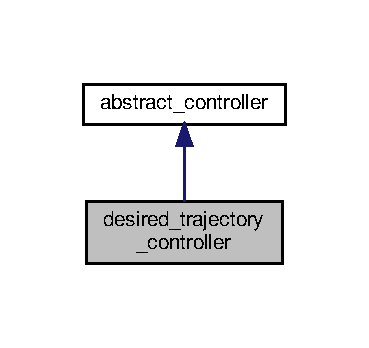
\includegraphics[width=177pt]{classdesired__trajectory__controller__inherit__graph}
\end{center}
\end{figure}


Collaboration diagram for desired\+\_\+trajectory\+\_\+controller\+:\nopagebreak
\begin{figure}[H]
\begin{center}
\leavevmode
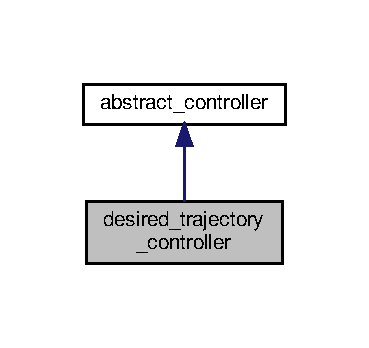
\includegraphics[width=177pt]{classdesired__trajectory__controller__coll__graph}
\end{center}
\end{figure}
\subsection*{Public Member Functions}
\begin{DoxyCompactItemize}
\item 
\mbox{\Hypertarget{classdesired__trajectory__controller_a42f8709a5746225c11b986d4587be874}\label{classdesired__trajectory__controller_a42f8709a5746225c11b986d4587be874}} 
std\+::vector$<$ double $>$ {\bfseries trajectory\+\_\+desired} (std\+::vector$<$ double $>$ barycenter, unsigned int l, unsigned int m, unsigned int n, unsigned int o)
\item 
\mbox{\Hypertarget{classdesired__trajectory__controller_a631fe1886a690d80364457fec3dfca86}\label{classdesired__trajectory__controller_a631fe1886a690d80364457fec3dfca86}} 
std\+::vector$<$ double $>$ {\bfseries trajectory\+\_\+desired\+\_\+harmonic\+\_\+oscillation} (std\+::vector$<$ double $>$ barycenter, unsigned int l, unsigned int m, unsigned int n, unsigned int o)
\item 
\mbox{\Hypertarget{classdesired__trajectory__controller_aa53734f2e492ea493b228bbf7518c421}\label{classdesired__trajectory__controller_aa53734f2e492ea493b228bbf7518c421}} 
std\+::vector$<$ double $>$ {\bfseries trajectory\+\_\+desired\+\_\+concentrating\+\_\+mean} (std\+::vector$<$ double $>$ barycenter, unsigned int l, unsigned int m, unsigned int n, unsigned int o)
\item 
\mbox{\Hypertarget{classdesired__trajectory__controller_a419e99f0f6be54bbba4b68bb0e45bf32}\label{classdesired__trajectory__controller_a419e99f0f6be54bbba4b68bb0e45bf32}} 
std\+::vector$<$ double $>$ {\bfseries trajectory\+\_\+desired\+\_\+shifting\+\_\+halfbox} (std\+::vector$<$ double $>$ barycenter, unsigned int l, unsigned int m, unsigned int n, unsigned int o)
\item 
\mbox{\Hypertarget{classdesired__trajectory__controller_ace11aeb778e779d8a7dc2eddec4c4a9d}\label{classdesired__trajectory__controller_ace11aeb778e779d8a7dc2eddec4c4a9d}} 
std\+::vector$<$ double $>$ {\bfseries trajectory\+\_\+desired\+\_\+concentrating\+\_\+center} (std\+::vector$<$ double $>$ barycenter, unsigned int l, unsigned int m, unsigned int n, unsigned int o)
\end{DoxyCompactItemize}


The documentation for this class was generated from the following files\+:\begin{DoxyCompactItemize}
\item 
/home/jan/\+Promotion\+\_\+linux\+P\+C/\+Optim\+\_\+\+V\+S\+T\+R\+A\+P/src/controller/desired\+\_\+trajectory\+\_\+controller.\+h\item 
/home/jan/\+Promotion\+\_\+linux\+P\+C/\+Optim\+\_\+\+V\+S\+T\+R\+A\+P/src/controller/desired\+\_\+trajectory\+\_\+controller.\+cpp\end{DoxyCompactItemize}

\hypertarget{classequation__solving__controller}{}\section{equation\+\_\+solving\+\_\+controller Class Reference}
\label{classequation__solving__controller}\index{equation\+\_\+solving\+\_\+controller@{equation\+\_\+solving\+\_\+controller}}


Inheritance diagram for equation\+\_\+solving\+\_\+controller\+:\nopagebreak
\begin{figure}[H]
\begin{center}
\leavevmode
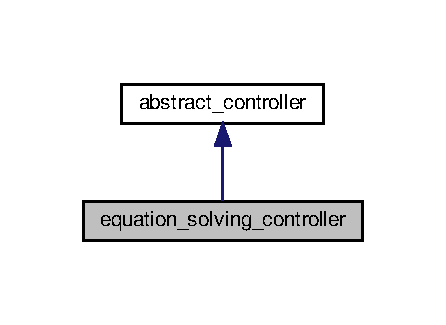
\includegraphics[width=214pt]{classequation__solving__controller__inherit__graph}
\end{center}
\end{figure}


Collaboration diagram for equation\+\_\+solving\+\_\+controller\+:\nopagebreak
\begin{figure}[H]
\begin{center}
\leavevmode
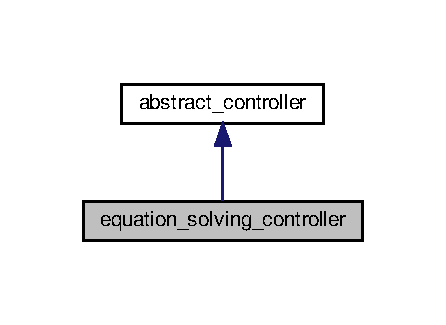
\includegraphics[width=214pt]{classequation__solving__controller__coll__graph}
\end{center}
\end{figure}
\subsection*{Public Member Functions}
\begin{DoxyCompactItemize}
\item 
\mbox{\Hypertarget{classequation__solving__controller_a281a20e8a2bb4b0b63f839ffbfea51b3}\label{classequation__solving__controller_a281a20e8a2bb4b0b63f839ffbfea51b3}} 
int {\bfseries start\+\_\+solving\+\_\+forward} (std\+::string start\+\_\+forward)
\item 
\mbox{\Hypertarget{classequation__solving__controller_a549c5c85c794cf0e7fbeacc3600fd830}\label{classequation__solving__controller_a549c5c85c794cf0e7fbeacc3600fd830}} 
int {\bfseries start\+\_\+solving\+\_\+backward} (std\+::string start\+\_\+backward)
\item 
\mbox{\Hypertarget{classequation__solving__controller_a3488080edc0c9a8cf8579fcd466ca429}\label{classequation__solving__controller_a3488080edc0c9a8cf8579fcd466ca429}} 
arma\+::mat {\bfseries Laplacian\+\_\+3D} ()
\item 
\mbox{\Hypertarget{classequation__solving__controller_a3ecc85d3b88fd0350ed0af025638de1c}\label{classequation__solving__controller_a3ecc85d3b88fd0350ed0af025638de1c}} 
arma\+::mat {\bfseries Laplacian\+\_\+\+Squared\+\_\+3D} ()
\end{DoxyCompactItemize}


The documentation for this class was generated from the following files\+:\begin{DoxyCompactItemize}
\item 
/home/jan/\+Promotion\+\_\+linux\+P\+C/\+Optim\+\_\+\+V\+S\+T\+R\+A\+P/src/controller/equation\+\_\+solving\+\_\+controller.\+h\item 
/home/jan/\+Promotion\+\_\+linux\+P\+C/\+Optim\+\_\+\+V\+S\+T\+R\+A\+P/src/controller/equation\+\_\+solving\+\_\+controller.\+cpp\end{DoxyCompactItemize}

\hypertarget{classgradient__calculator}{}\section{gradient\+\_\+calculator Class Reference}
\label{classgradient__calculator}\index{gradient\+\_\+calculator@{gradient\+\_\+calculator}}


Inheritance diagram for gradient\+\_\+calculator\+:\nopagebreak
\begin{figure}[H]
\begin{center}
\leavevmode
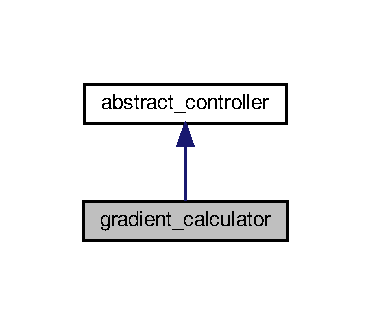
\includegraphics[width=178pt]{classgradient__calculator__inherit__graph}
\end{center}
\end{figure}


Collaboration diagram for gradient\+\_\+calculator\+:\nopagebreak
\begin{figure}[H]
\begin{center}
\leavevmode
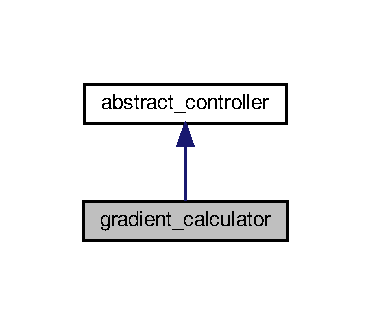
\includegraphics[width=178pt]{classgradient__calculator__coll__graph}
\end{center}
\end{figure}
\subsection*{Public Member Functions}
\begin{DoxyCompactItemize}
\item 
\mbox{\Hypertarget{classgradient__calculator_a811af658cf499119c6f00e6457880824}\label{classgradient__calculator_a811af658cf499119c6f00e6457880824}} 
{\bfseries gradient\+\_\+calculator} (const char $\ast$filename)
\item 
\mbox{\Hypertarget{classgradient__calculator_a087141d845a78621543e127a1e180809}\label{classgradient__calculator_a087141d845a78621543e127a1e180809}} 
arma\+::mat {\bfseries calculate\+Gradient\+\_\+force\+Control\+\_\+space\+\_\+\+L2} (std\+::vector$<$ std\+::unordered\+\_\+map$<$ \hyperlink{classcoordinate__phase__space__time}{coordinate\+\_\+phase\+\_\+space\+\_\+time}, double $>$$>$ forward\+P\+D\+F\+\_\+time, std\+::vector$<$ std\+::unordered\+\_\+map$<$ \hyperlink{classcoordinate__phase__space__time}{coordinate\+\_\+phase\+\_\+space\+\_\+time}, double $>$$>$ backward\+P\+D\+F\+\_\+time, arma\+::mat control)
\item 
\mbox{\Hypertarget{classgradient__calculator_a8381a8497dfe88bcb04ff40ce1e235e0}\label{classgradient__calculator_a8381a8497dfe88bcb04ff40ce1e235e0}} 
arma\+::mat {\bfseries calculate\+Gradient\+\_\+force\+Control\+\_\+space\+\_\+\+Hm} (std\+::vector$<$ std\+::unordered\+\_\+map$<$ \hyperlink{classcoordinate__phase__space__time}{coordinate\+\_\+phase\+\_\+space\+\_\+time}, double $>$$>$ forward\+P\+D\+F\+\_\+time, std\+::vector$<$ std\+::unordered\+\_\+map$<$ \hyperlink{classcoordinate__phase__space__time}{coordinate\+\_\+phase\+\_\+space\+\_\+time}, double $>$$>$ backward\+P\+D\+F\+\_\+time, arma\+::mat control)
\end{DoxyCompactItemize}


The documentation for this class was generated from the following files\+:\begin{DoxyCompactItemize}
\item 
/home/jan/\+Promotion\+\_\+linux\+P\+C/\+Optim\+\_\+\+V\+S\+T\+R\+A\+P/src/optimization/gradient\+\_\+calculator.\+h\item 
/home/jan/\+Promotion\+\_\+linux\+P\+C/\+Optim\+\_\+\+V\+S\+T\+R\+A\+P/src/optimization/gradient\+\_\+calculator.\+cpp\end{DoxyCompactItemize}

\hypertarget{structstd_1_1hash_3_01coordinate__phase__space__time_01_4}{}\section{std\+:\+:hash$<$ coordinate\+\_\+phase\+\_\+space\+\_\+time $>$ Struct Template Reference}
\label{structstd_1_1hash_3_01coordinate__phase__space__time_01_4}\index{std\+::hash$<$ coordinate\+\_\+phase\+\_\+space\+\_\+time $>$@{std\+::hash$<$ coordinate\+\_\+phase\+\_\+space\+\_\+time $>$}}
\subsection*{Public Types}
\begin{DoxyCompactItemize}
\item 
\mbox{\Hypertarget{structstd_1_1hash_3_01coordinate__phase__space__time_01_4_a1ece1aa71d27828da1dfe89ef9148c89}\label{structstd_1_1hash_3_01coordinate__phase__space__time_01_4_a1ece1aa71d27828da1dfe89ef9148c89}} 
typedef \hyperlink{classcoordinate__phase__space__time}{coordinate\+\_\+phase\+\_\+space\+\_\+time} {\bfseries argument\+\_\+type}
\item 
\mbox{\Hypertarget{structstd_1_1hash_3_01coordinate__phase__space__time_01_4_aee0af0c5edc703ce2958d3e03e9692b7}\label{structstd_1_1hash_3_01coordinate__phase__space__time_01_4_aee0af0c5edc703ce2958d3e03e9692b7}} 
typedef size\+\_\+t {\bfseries result\+\_\+type}
\end{DoxyCompactItemize}
\subsection*{Public Member Functions}
\begin{DoxyCompactItemize}
\item 
\mbox{\Hypertarget{structstd_1_1hash_3_01coordinate__phase__space__time_01_4_a09402ca0b8c7669cced9eeca29d291e8}\label{structstd_1_1hash_3_01coordinate__phase__space__time_01_4_a09402ca0b8c7669cced9eeca29d291e8}} 
size\+\_\+t {\bfseries operator()} (const \hyperlink{classcoordinate__phase__space__time}{argument\+\_\+type} \&x) const
\end{DoxyCompactItemize}


The documentation for this struct was generated from the following file\+:\begin{DoxyCompactItemize}
\item 
/home/jan/\+Promotion\+\_\+linux\+P\+C/\+Optim\+\_\+\+V\+S\+T\+R\+A\+P/src/objects/coordinate\+\_\+phase\+\_\+space\+\_\+time.\+h\end{DoxyCompactItemize}

\hypertarget{classinput}{}\section{input Class Reference}
\label{classinput}\index{input@{input}}


Inheritance diagram for input\+:\nopagebreak
\begin{figure}[H]
\begin{center}
\leavevmode
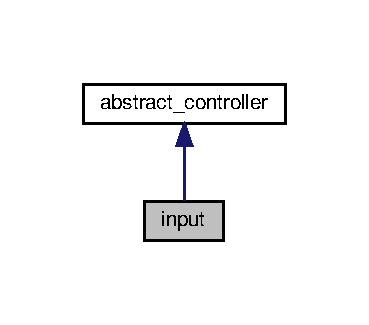
\includegraphics[width=177pt]{classinput__inherit__graph}
\end{center}
\end{figure}


Collaboration diagram for input\+:\nopagebreak
\begin{figure}[H]
\begin{center}
\leavevmode
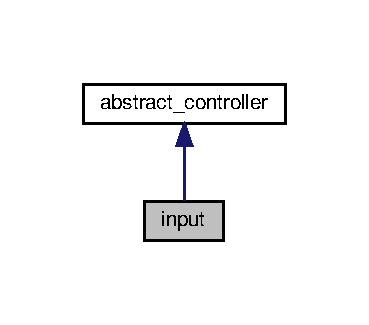
\includegraphics[width=177pt]{classinput__coll__graph}
\end{center}
\end{figure}
\subsection*{Public Member Functions}
\begin{DoxyCompactItemize}
\item 
\mbox{\Hypertarget{classinput_a26c2b30593898a6ad3806d3e548f6002}\label{classinput_a26c2b30593898a6ad3806d3e548f6002}} 
unsigned int {\bfseries read\+\_\+plasma\+\_\+state\+\_\+forward} (std\+::vector$<$ std\+::vector$<$ \hyperlink{classparticle}{particle} $>$$>$ \&forward\+Particles)
\item 
\mbox{\Hypertarget{classinput_a9b874ae8e6cdc97cb9b2d2989aa26a68}\label{classinput_a9b874ae8e6cdc97cb9b2d2989aa26a68}} 
unsigned int {\bfseries read\+\_\+plasma\+\_\+state\+\_\+backward} (std\+::vector$<$ std\+::vector$<$ \hyperlink{classparticle}{particle} $>$$>$ \&backward\+Particles)
\end{DoxyCompactItemize}
\subsection*{Static Public Member Functions}
\begin{DoxyCompactItemize}
\item 
\mbox{\Hypertarget{classinput_aa52f1efda75b6a38b8058ec4731e4a5c}\label{classinput_aa52f1efda75b6a38b8058ec4731e4a5c}} 
static std\+::vector$<$ \hyperlink{classparticle}{particle} $>$ {\bfseries read\+Particle\+Vector} (std\+::string filename, std\+::string delimiter)
\item 
\mbox{\Hypertarget{classinput_abc407f396e45ac72844e65cb73cfb335}\label{classinput_abc407f396e45ac72844e65cb73cfb335}} 
static arma\+::mat {\bfseries read\+Control} (const char $\ast$filename)
\end{DoxyCompactItemize}


The documentation for this class was generated from the following files\+:\begin{DoxyCompactItemize}
\item 
/home/jan/\+Promotion\+\_\+linux\+P\+C/\+Optim\+\_\+\+V\+S\+T\+R\+A\+P/src/io/input.\+h\item 
/home/jan/\+Promotion\+\_\+linux\+P\+C/\+Optim\+\_\+\+V\+S\+T\+R\+A\+P/src/io/input.\+cpp\end{DoxyCompactItemize}

\hypertarget{classmesh_1_1Mesh}{}\section{mesh.\+Mesh Class Reference}
\label{classmesh_1_1Mesh}\index{mesh.\+Mesh@{mesh.\+Mesh}}
\subsection*{Public Member Functions}
\begin{DoxyCompactItemize}
\item 
\mbox{\Hypertarget{classmesh_1_1Mesh_addb129a90452df779740275c9e97b2ee}\label{classmesh_1_1Mesh_addb129a90452df779740275c9e97b2ee}} 
def {\bfseries \+\_\+\+\_\+init\+\_\+\+\_\+} (self)
\item 
\mbox{\Hypertarget{classmesh_1_1Mesh_a0e3c8b565fd6502b16cd2c075e861635}\label{classmesh_1_1Mesh_a0e3c8b565fd6502b16cd2c075e861635}} 
def {\bfseries \+\_\+\+\_\+str\+\_\+\+\_\+} (self)
\item 
\mbox{\Hypertarget{classmesh_1_1Mesh_a7140e72e3b248afaf1fbe5791bd07679}\label{classmesh_1_1Mesh_a7140e72e3b248afaf1fbe5791bd07679}} 
def {\bfseries clear} (self)
\item 
\mbox{\Hypertarget{classmesh_1_1Mesh_a7aff8aa8badefcb845890649cd54dc8d}\label{classmesh_1_1Mesh_a7aff8aa8badefcb845890649cd54dc8d}} 
def {\bfseries read\+\_\+mesh\+\_\+xml} (self, file\+\_\+name)
\item 
\mbox{\Hypertarget{classmesh_1_1Mesh_a512a630d8e15f8a5acbfff07d87b9dd9}\label{classmesh_1_1Mesh_a512a630d8e15f8a5acbfff07d87b9dd9}} 
def {\bfseries interpolate\+\_\+cell2node} (self)
\item 
\mbox{\Hypertarget{classmesh_1_1Mesh_afc4ba44d2c3ca4fb318d8c5ab28d7cff}\label{classmesh_1_1Mesh_afc4ba44d2c3ca4fb318d8c5ab28d7cff}} 
def {\bfseries read\+\_\+control\+\_\+csv} (self, file\+\_\+name)
\item 
\mbox{\Hypertarget{classmesh_1_1Mesh_a0d86fdca66e4582ffc1b85502375f1cd}\label{classmesh_1_1Mesh_a0d86fdca66e4582ffc1b85502375f1cd}} 
def {\bfseries read\+\_\+control\+\_\+xml} (self, file\+\_\+name)
\item 
\mbox{\Hypertarget{classmesh_1_1Mesh_a01ac5a14c6d0998317f619ac16d0f9f6}\label{classmesh_1_1Mesh_a01ac5a14c6d0998317f619ac16d0f9f6}} 
def {\bfseries write\+\_\+control\+\_\+csv} (self, file\+\_\+name)
\item 
\mbox{\Hypertarget{classmesh_1_1Mesh_a33b2b5cf4e35bfe44407eef364de3141}\label{classmesh_1_1Mesh_a33b2b5cf4e35bfe44407eef364de3141}} 
def {\bfseries write\+\_\+control\+\_\+xml} (self, file\+\_\+name)
\item 
\mbox{\Hypertarget{classmesh_1_1Mesh_a41a3e2655e1c79c6aca6776693f209e6}\label{classmesh_1_1Mesh_a41a3e2655e1c79c6aca6776693f209e6}} 
def {\bfseries write\+\_\+barycenters\+\_\+xml} (self, file\+\_\+name)
\end{DoxyCompactItemize}
\subsection*{Public Attributes}
\begin{DoxyCompactItemize}
\item 
\mbox{\Hypertarget{classmesh_1_1Mesh_aae2a3fbf55b22d4bccd0ce83cc11be57}\label{classmesh_1_1Mesh_aae2a3fbf55b22d4bccd0ce83cc11be57}} 
{\bfseries cells}
\item 
\mbox{\Hypertarget{classmesh_1_1Mesh_a22bcb6ef348b8291241cd95c27e1ba66}\label{classmesh_1_1Mesh_a22bcb6ef348b8291241cd95c27e1ba66}} 
{\bfseries nodes}
\item 
\mbox{\Hypertarget{classmesh_1_1Mesh_a101a440d5b02561a06dde8662cf69f54}\label{classmesh_1_1Mesh_a101a440d5b02561a06dde8662cf69f54}} 
{\bfseries volume}
\end{DoxyCompactItemize}


The documentation for this class was generated from the following file\+:\begin{DoxyCompactItemize}
\item 
/home/jan/\+Promotion\+\_\+linux\+P\+C/\+Optim\+\_\+\+V\+S\+T\+R\+A\+P/optim-\/vstrap-\/toolset/toolset/mesh.\+py\end{DoxyCompactItemize}

\hypertarget{classmesh_1_1MeshTest}{}\section{mesh.\+Mesh\+Test Class Reference}
\label{classmesh_1_1MeshTest}\index{mesh.\+Mesh\+Test@{mesh.\+Mesh\+Test}}


Inheritance diagram for mesh.\+Mesh\+Test\+:\nopagebreak
\begin{figure}[H]
\begin{center}
\leavevmode
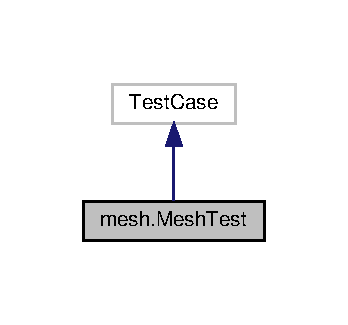
\includegraphics[width=167pt]{classmesh_1_1MeshTest__inherit__graph}
\end{center}
\end{figure}


Collaboration diagram for mesh.\+Mesh\+Test\+:\nopagebreak
\begin{figure}[H]
\begin{center}
\leavevmode
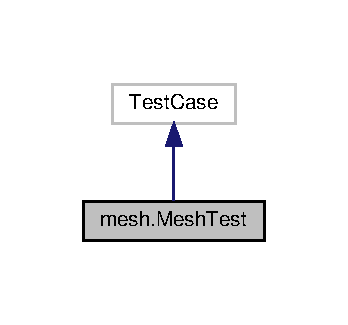
\includegraphics[width=167pt]{classmesh_1_1MeshTest__coll__graph}
\end{center}
\end{figure}
\subsection*{Public Member Functions}
\begin{DoxyCompactItemize}
\item 
\mbox{\Hypertarget{classmesh_1_1MeshTest_aadbea4688c34405d93e63a73744d3b49}\label{classmesh_1_1MeshTest_aadbea4688c34405d93e63a73744d3b49}} 
def {\bfseries test\+\_\+read\+\_\+mesh\+\_\+xml} (self)
\item 
\mbox{\Hypertarget{classmesh_1_1MeshTest_a72429959940aca2333822a686964b29c}\label{classmesh_1_1MeshTest_a72429959940aca2333822a686964b29c}} 
def {\bfseries test\+\_\+read\+\_\+control\+\_\+csv} (self)
\item 
\mbox{\Hypertarget{classmesh_1_1MeshTest_a409b1c2216946515c4c50bcfc4b9dee3}\label{classmesh_1_1MeshTest_a409b1c2216946515c4c50bcfc4b9dee3}} 
def {\bfseries test\+\_\+read\+\_\+control\+\_\+xml} (self)
\item 
\mbox{\Hypertarget{classmesh_1_1MeshTest_a38f39aaad1915bc5ebde163699ac7485}\label{classmesh_1_1MeshTest_a38f39aaad1915bc5ebde163699ac7485}} 
def {\bfseries test\+\_\+interpolate\+\_\+cell2node} (self)
\end{DoxyCompactItemize}


The documentation for this class was generated from the following file\+:\begin{DoxyCompactItemize}
\item 
/home/jan/\+Promotion\+\_\+linux\+P\+C/\+Optim\+\_\+\+V\+S\+T\+R\+A\+P/optim-\/vstrap-\/toolset/tests/mesh.\+py\end{DoxyCompactItemize}

\hypertarget{classmesh_1_1Node}{}\section{mesh.\+Node Class Reference}
\label{classmesh_1_1Node}\index{mesh.\+Node@{mesh.\+Node}}
\subsection*{Public Member Functions}
\begin{DoxyCompactItemize}
\item 
\mbox{\Hypertarget{classmesh_1_1Node_a3217d462af12c56ef6ada880de4a478f}\label{classmesh_1_1Node_a3217d462af12c56ef6ada880de4a478f}} 
def {\bfseries \+\_\+\+\_\+init\+\_\+\+\_\+} (self, id=0, coord=(0.\+0, 0.\+0, 0.\+0))
\item 
\mbox{\Hypertarget{classmesh_1_1Node_a96903bf25e248be9051c9f0aa3772fd7}\label{classmesh_1_1Node_a96903bf25e248be9051c9f0aa3772fd7}} 
def {\bfseries get\+\_\+position} (self)
\end{DoxyCompactItemize}
\subsection*{Public Attributes}
\begin{DoxyCompactItemize}
\item 
\mbox{\Hypertarget{classmesh_1_1Node_ad8e114d00c3d58afe2cfc0faf8460563}\label{classmesh_1_1Node_ad8e114d00c3d58afe2cfc0faf8460563}} 
{\bfseries id}
\item 
\mbox{\Hypertarget{classmesh_1_1Node_a327f78d3114ec42494d876bb17dfb069}\label{classmesh_1_1Node_a327f78d3114ec42494d876bb17dfb069}} 
{\bfseries x\+\_\+coord}
\item 
\mbox{\Hypertarget{classmesh_1_1Node_a27250f449af1f16d9f50c5dfca7f93cf}\label{classmesh_1_1Node_a27250f449af1f16d9f50c5dfca7f93cf}} 
{\bfseries y\+\_\+coord}
\item 
\mbox{\Hypertarget{classmesh_1_1Node_a8c3a747344f22f916f76f35586645fd0}\label{classmesh_1_1Node_a8c3a747344f22f916f76f35586645fd0}} 
{\bfseries z\+\_\+coord}
\item 
\mbox{\Hypertarget{classmesh_1_1Node_a64b90f8937228522c25eada3fbfc3f05}\label{classmesh_1_1Node_a64b90f8937228522c25eada3fbfc3f05}} 
{\bfseries value}
\end{DoxyCompactItemize}


The documentation for this class was generated from the following file\+:\begin{DoxyCompactItemize}
\item 
/home/jan/\+Promotion\+\_\+linux\+P\+C/\+Optim\+\_\+\+V\+S\+T\+R\+A\+P/optim-\/vstrap-\/toolset/toolset/mesh.\+py\end{DoxyCompactItemize}

\hypertarget{classobjective__calculator}{}\section{objective\+\_\+calculator Class Reference}
\label{classobjective__calculator}\index{objective\+\_\+calculator@{objective\+\_\+calculator}}


Inheritance diagram for objective\+\_\+calculator\+:\nopagebreak
\begin{figure}[H]
\begin{center}
\leavevmode
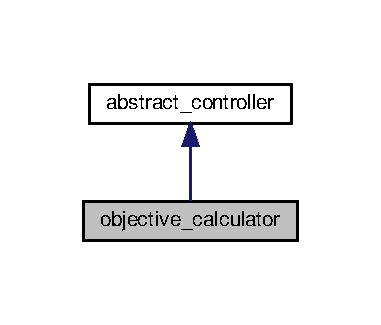
\includegraphics[width=183pt]{classobjective__calculator__inherit__graph}
\end{center}
\end{figure}


Collaboration diagram for objective\+\_\+calculator\+:\nopagebreak
\begin{figure}[H]
\begin{center}
\leavevmode
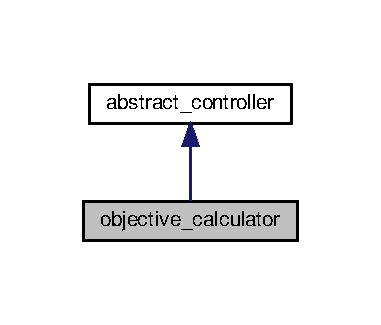
\includegraphics[width=183pt]{classobjective__calculator__coll__graph}
\end{center}
\end{figure}
\subsection*{Public Member Functions}
\begin{DoxyCompactItemize}
\item 
\mbox{\Hypertarget{classobjective__calculator_ac0122306f4282be07f42f38d761a4bff}\label{classobjective__calculator_ac0122306f4282be07f42f38d761a4bff}} 
{\bfseries objective\+\_\+calculator} (const char $\ast$filename)
\item 
\mbox{\Hypertarget{classobjective__calculator_ac0d0237d5f738a90abc4492220134784}\label{classobjective__calculator_ac0d0237d5f738a90abc4492220134784}} 
double {\bfseries calculate\+\_\+objective\+\_\+\+L2} (std\+::vector$<$ std\+::unordered\+\_\+map$<$ \hyperlink{classcoordinate__phase__space__time}{coordinate\+\_\+phase\+\_\+space\+\_\+time}, double $>$$>$ forward\+P\+D\+F\+\_\+time, arma\+::mat control)
\end{DoxyCompactItemize}


The documentation for this class was generated from the following files\+:\begin{DoxyCompactItemize}
\item 
/home/jan/\+Promotion\+\_\+linux\+P\+C/\+Optim\+\_\+\+V\+S\+T\+R\+A\+P/src/optimization/objective\+\_\+calculator.\+h\item 
/home/jan/\+Promotion\+\_\+linux\+P\+C/\+Optim\+\_\+\+V\+S\+T\+R\+A\+P/src/optimization/objective\+\_\+calculator.\+cpp\end{DoxyCompactItemize}

\hypertarget{classoptim__controller}{}\section{optim\+\_\+controller Class Reference}
\label{classoptim__controller}\index{optim\+\_\+controller@{optim\+\_\+controller}}


Inheritance diagram for optim\+\_\+controller\+:\nopagebreak
\begin{figure}[H]
\begin{center}
\leavevmode
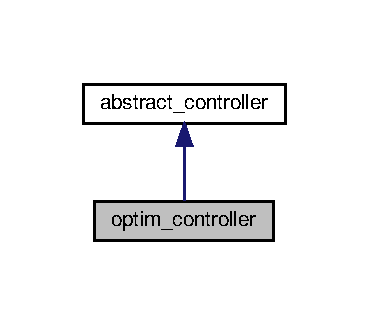
\includegraphics[width=177pt]{classoptim__controller__inherit__graph}
\end{center}
\end{figure}


Collaboration diagram for optim\+\_\+controller\+:\nopagebreak
\begin{figure}[H]
\begin{center}
\leavevmode
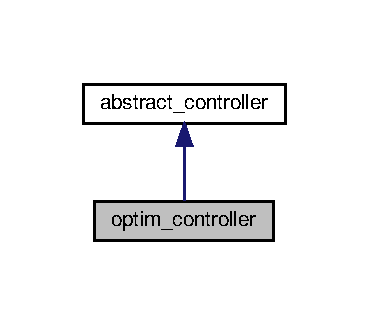
\includegraphics[width=177pt]{classoptim__controller__coll__graph}
\end{center}
\end{figure}
\subsection*{Public Member Functions}
\begin{DoxyCompactItemize}
\item 
\mbox{\Hypertarget{classoptim__controller_a239f21ed616ef8f350b386cea9be81c1}\label{classoptim__controller_a239f21ed616ef8f350b386cea9be81c1}} 
int {\bfseries start\+\_\+optimizer} (int argc, const char $\ast$$\ast$argv)
\end{DoxyCompactItemize}
\subsection*{Static Public Member Functions}
\begin{DoxyCompactItemize}
\item 
static int \hyperlink{classoptim__controller_abbf7841344a99ccd29fc38891763b43f}{start\+\_\+optimization\+\_\+iteration} (const char $\ast$input\+\_\+xml\+\_\+path)
\item 
\mbox{\Hypertarget{classoptim__controller_a59a2704ba13f6d865de66c6df1838ef7}\label{classoptim__controller_a59a2704ba13f6d865de66c6df1838ef7}} 
static std\+::unordered\+\_\+map$<$ \hyperlink{classcoordinate__phase__space__time}{coordinate\+\_\+phase\+\_\+space\+\_\+time}, double $>$ {\bfseries assemble\+P\+D\+F\+\_\+thread} (std\+::vector$<$ std\+::vector$<$ \hyperlink{classparticle}{particle} $>$$>$ \&particles, unsigned int equation\+\_\+type, \hyperlink{classdata__provider}{data\+\_\+provider} data\+\_\+provider\+\_\+)
\item 
\mbox{\Hypertarget{classoptim__controller_a0b0264fedf364aca6d7531fb54239f10}\label{classoptim__controller_a0b0264fedf364aca6d7531fb54239f10}} 
static int {\bfseries check\+\_\+input\+\_\+py} (\hyperlink{classdata__provider}{data\+\_\+provider} provider, const char $\ast$file\+Path\+Optim\+Input)
\item 
\mbox{\Hypertarget{classoptim__controller_af1012e1ce21abe7056d3a48ce1c58c1e}\label{classoptim__controller_af1012e1ce21abe7056d3a48ce1c58c1e}} 
static int {\bfseries interpolate\+\_\+control} (\hyperlink{classdata__provider}{data\+\_\+provider} provider)
\item 
\mbox{\Hypertarget{classoptim__controller_a97a287ae5ad640cc535a5cb3c1daad7f}\label{classoptim__controller_a97a287ae5ad640cc535a5cb3c1daad7f}} 
static arma\+::mat {\bfseries start\+\_\+with\+\_\+zero\+\_\+control} (const char $\ast$input\+\_\+xml\+\_\+path)
\item 
\mbox{\Hypertarget{classoptim__controller_a13e9d1f3242d17fb59bdb7c3f3cec85a}\label{classoptim__controller_a13e9d1f3242d17fb59bdb7c3f3cec85a}} 
static arma\+::mat {\bfseries start\+\_\+with\+\_\+given\+\_\+control} (const char $\ast$input\+\_\+xml\+\_\+path)
\end{DoxyCompactItemize}


\subsection{Member Function Documentation}
\mbox{\Hypertarget{classoptim__controller_abbf7841344a99ccd29fc38891763b43f}\label{classoptim__controller_abbf7841344a99ccd29fc38891763b43f}} 
\index{optim\+\_\+controller@{optim\+\_\+controller}!start\+\_\+optimization\+\_\+iteration@{start\+\_\+optimization\+\_\+iteration}}
\index{start\+\_\+optimization\+\_\+iteration@{start\+\_\+optimization\+\_\+iteration}!optim\+\_\+controller@{optim\+\_\+controller}}
\subsubsection{\texorpdfstring{start\+\_\+optimization\+\_\+iteration()}{start\_optimization\_iteration()}}
{\footnotesize\ttfamily int optim\+\_\+controller\+::start\+\_\+optimization\+\_\+iteration (\begin{DoxyParamCaption}\item[{const char $\ast$}]{input\+\_\+xml\+\_\+path }\end{DoxyParamCaption})\hspace{0.3cm}{\ttfamily [static]}}

S\+T\+A\+RT O\+P\+T\+I\+M\+I\+Z\+A\+T\+I\+ON I\+T\+E\+R\+A\+T\+I\+ONHere is the call graph for this function\+:\nopagebreak
\begin{figure}[H]
\begin{center}
\leavevmode
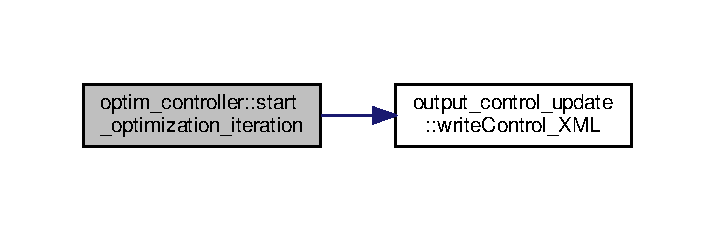
\includegraphics[width=343pt]{classoptim__controller_abbf7841344a99ccd29fc38891763b43f_cgraph}
\end{center}
\end{figure}


The documentation for this class was generated from the following files\+:\begin{DoxyCompactItemize}
\item 
/home/jan/\+Promotion\+\_\+linux\+P\+C/\+Optim\+\_\+\+V\+S\+T\+R\+A\+P/src/controller/optim\+\_\+controller.\+h\item 
/home/jan/\+Promotion\+\_\+linux\+P\+C/\+Optim\+\_\+\+V\+S\+T\+R\+A\+P/src/controller/optim\+\_\+controller.\+cpp\end{DoxyCompactItemize}

\hypertarget{classoutput__control__update}{}\section{output\+\_\+control\+\_\+update Class Reference}
\label{classoutput__control__update}\index{output\+\_\+control\+\_\+update@{output\+\_\+control\+\_\+update}}


The \hyperlink{classoutput__control__update}{output\+\_\+control\+\_\+update} class offers functions to write the update of the control in a file that is readable by the solver for forward and backward equation.  




{\ttfamily \#include $<$output\+\_\+control\+\_\+update.\+h$>$}



Inheritance diagram for output\+\_\+control\+\_\+update\+:\nopagebreak
\begin{figure}[H]
\begin{center}
\leavevmode
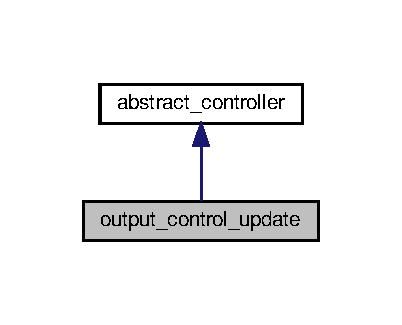
\includegraphics[width=193pt]{classoutput__control__update__inherit__graph}
\end{center}
\end{figure}


Collaboration diagram for output\+\_\+control\+\_\+update\+:\nopagebreak
\begin{figure}[H]
\begin{center}
\leavevmode
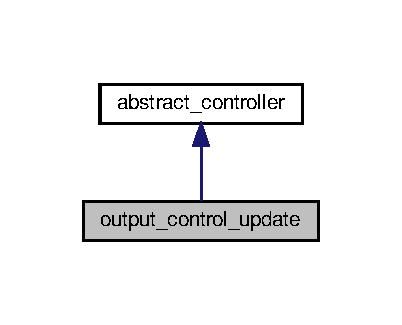
\includegraphics[width=193pt]{classoutput__control__update__coll__graph}
\end{center}
\end{figure}
\subsection*{Public Member Functions}
\begin{DoxyCompactItemize}
\item 
\mbox{\Hypertarget{classoutput__control__update_a1e74afe80e283735d4392d8e58c81d40}\label{classoutput__control__update_a1e74afe80e283735d4392d8e58c81d40}} 
{\bfseries output\+\_\+control\+\_\+update} (const char $\ast$filename)
\item 
int \hyperlink{classoutput__control__update_a8261c07e1a6a3a34171ceecb93b27382}{write\+Control\+\_\+\+X\+ML} (arma\+::mat control)
\begin{DoxyCompactList}\small\item\em write\+Control\+\_\+\+X\+ML takes a control and writes a corresponding X\+ML file \end{DoxyCompactList}\end{DoxyCompactItemize}


\subsection{Detailed Description}
The \hyperlink{classoutput__control__update}{output\+\_\+control\+\_\+update} class offers functions to write the update of the control in a file that is readable by the solver for forward and backward equation. 

\subsection{Member Function Documentation}
\mbox{\Hypertarget{classoutput__control__update_a8261c07e1a6a3a34171ceecb93b27382}\label{classoutput__control__update_a8261c07e1a6a3a34171ceecb93b27382}} 
\index{output\+\_\+control\+\_\+update@{output\+\_\+control\+\_\+update}!write\+Control\+\_\+\+X\+ML@{write\+Control\+\_\+\+X\+ML}}
\index{write\+Control\+\_\+\+X\+ML@{write\+Control\+\_\+\+X\+ML}!output\+\_\+control\+\_\+update@{output\+\_\+control\+\_\+update}}
\subsubsection{\texorpdfstring{write\+Control\+\_\+\+X\+M\+L()}{writeControl\_XML()}}
{\footnotesize\ttfamily int output\+\_\+control\+\_\+update\+::write\+Control\+\_\+\+X\+ML (\begin{DoxyParamCaption}\item[{arma\+::mat}]{control }\end{DoxyParamCaption})}



write\+Control\+\_\+\+X\+ML takes a control and writes a corresponding X\+ML file 


\begin{DoxyParams}{Parameters}
{\em control} & (arma\+::mat) \\
\hline
\end{DoxyParams}
\begin{DoxyReturn}{Returns}
0 if process successfully 
\end{DoxyReturn}


The documentation for this class was generated from the following files\+:\begin{DoxyCompactItemize}
\item 
/home/jan/\+Promotion\+\_\+linux\+P\+C/\+Optim\+\_\+\+V\+S\+T\+R\+A\+P/src/io/output\+\_\+control\+\_\+update.\+h\item 
/home/jan/\+Promotion\+\_\+linux\+P\+C/\+Optim\+\_\+\+V\+S\+T\+R\+A\+P/src/io/output\+\_\+control\+\_\+update.\+cpp\end{DoxyCompactItemize}

\hypertarget{classoutput__diagnostics}{}\section{output\+\_\+diagnostics Class Reference}
\label{classoutput__diagnostics}\index{output\+\_\+diagnostics@{output\+\_\+diagnostics}}


Inheritance diagram for output\+\_\+diagnostics\+:\nopagebreak
\begin{figure}[H]
\begin{center}
\leavevmode
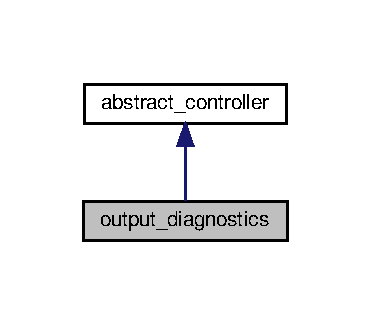
\includegraphics[width=178pt]{classoutput__diagnostics__inherit__graph}
\end{center}
\end{figure}


Collaboration diagram for output\+\_\+diagnostics\+:\nopagebreak
\begin{figure}[H]
\begin{center}
\leavevmode
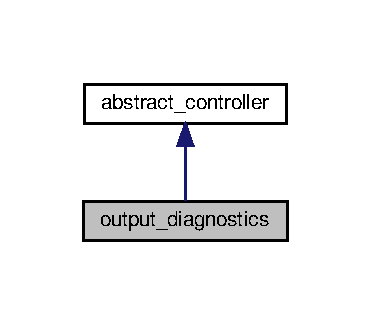
\includegraphics[width=178pt]{classoutput__diagnostics__coll__graph}
\end{center}
\end{figure}
\subsection*{Public Member Functions}
\begin{DoxyCompactItemize}
\item 
\mbox{\Hypertarget{classoutput__diagnostics_a397079340ca3f8f1d03d46221739c542}\label{classoutput__diagnostics_a397079340ca3f8f1d03d46221739c542}} 
int {\bfseries write\+Gradient\+To\+File} (arma\+::mat gradient, std\+::string filename)
\item 
\mbox{\Hypertarget{classoutput__diagnostics_a3c36ad7c103a2003087b501fc8dded79}\label{classoutput__diagnostics_a3c36ad7c103a2003087b501fc8dded79}} 
int {\bfseries write\+Double\+To\+File} (double value, std\+::string filename)
\end{DoxyCompactItemize}


The documentation for this class was generated from the following files\+:\begin{DoxyCompactItemize}
\item 
/home/jan/\+Promotion\+\_\+linux\+P\+C/\+Optim\+\_\+\+V\+S\+T\+R\+A\+P/src/io/output\+\_\+diagnostics.\+h\item 
/home/jan/\+Promotion\+\_\+linux\+P\+C/\+Optim\+\_\+\+V\+S\+T\+R\+A\+P/src/io/output\+\_\+diagnostics.\+cpp\end{DoxyCompactItemize}

\hypertarget{classparticle}{}\section{particle Class Reference}
\label{classparticle}\index{particle@{particle}}
\subsection*{Public Member Functions}
\begin{DoxyCompactItemize}
\item 
\mbox{\Hypertarget{classparticle_aa5adef29810de80b814f3d9938b4c9aa}\label{classparticle_aa5adef29810de80b814f3d9938b4c9aa}} 
{\bfseries particle} (double vx, double vy, double vz)
\item 
\mbox{\Hypertarget{classparticle_a9b729c767ff1da43dc1fe6bba898a710}\label{classparticle_a9b729c767ff1da43dc1fe6bba898a710}} 
{\bfseries particle} (double px, double py, double pz, double vx, double vy, double vz)
\item 
\mbox{\Hypertarget{classparticle_a19d2d4e8dc60c0a014415a601671bd07}\label{classparticle_a19d2d4e8dc60c0a014415a601671bd07}} 
{\bfseries particle} (double px, double py, double pz, double vx, double vy, double vz, int cell\+\_\+id)
\item 
\mbox{\Hypertarget{classparticle_ab743d68f73ebb2ae9fa18c05cf1a5bf3}\label{classparticle_ab743d68f73ebb2ae9fa18c05cf1a5bf3}} 
bool {\bfseries operator==} (const \hyperlink{classparticle}{particle} \&\hyperlink{classparticle}{particle}) const
\item 
double \hyperlink{classparticle_a4746319805ea7d18c4a3eac998b02043}{get\+Velocity\+Magnitude\+Particle} ()
\begin{DoxyCompactList}\small\item\em get\+Velocity\+Magnitude\+Particle calculates speed of particles using Euclidean Norm \end{DoxyCompactList}\item 
std\+::string \hyperlink{classparticle_a48098f62cff10f99c3676ac12a168f02}{to\+String} ()
\begin{DoxyCompactList}\small\item\em to\+String \end{DoxyCompactList}\item 
\mbox{\Hypertarget{classparticle_a932b36c4cdf7439e02f06ca764f9c286}\label{classparticle_a932b36c4cdf7439e02f06ca764f9c286}} 
double {\bfseries get\+Px} () const
\item 
\mbox{\Hypertarget{classparticle_a6d1bbc85ccbe0d7656d004419f65ef3f}\label{classparticle_a6d1bbc85ccbe0d7656d004419f65ef3f}} 
void {\bfseries set\+Px} (double value)
\item 
\mbox{\Hypertarget{classparticle_aeab6ac7d11e9b6bbb3a36a16e22f3f8a}\label{classparticle_aeab6ac7d11e9b6bbb3a36a16e22f3f8a}} 
double {\bfseries get\+Py} () const
\item 
\mbox{\Hypertarget{classparticle_ade3bada039b69771fae50f5f918a3cdb}\label{classparticle_ade3bada039b69771fae50f5f918a3cdb}} 
void {\bfseries set\+Py} (double value)
\item 
\mbox{\Hypertarget{classparticle_abc9f033b62a0b648155647537400f7f2}\label{classparticle_abc9f033b62a0b648155647537400f7f2}} 
double {\bfseries get\+Pz} () const
\item 
\mbox{\Hypertarget{classparticle_aa196f1416d69407ecca7f52a91247a68}\label{classparticle_aa196f1416d69407ecca7f52a91247a68}} 
void {\bfseries set\+Pz} (double value)
\item 
\mbox{\Hypertarget{classparticle_a3d8df6c15a3780de1d1bb65a0e9129a9}\label{classparticle_a3d8df6c15a3780de1d1bb65a0e9129a9}} 
double {\bfseries get\+Vx} () const
\item 
\mbox{\Hypertarget{classparticle_aafdf504b9f8dc712312140309711b091}\label{classparticle_aafdf504b9f8dc712312140309711b091}} 
void {\bfseries set\+Vx} (double value)
\item 
\mbox{\Hypertarget{classparticle_a6baa7233d3d1899efda70ceb9325552b}\label{classparticle_a6baa7233d3d1899efda70ceb9325552b}} 
double {\bfseries get\+Vy} () const
\item 
\mbox{\Hypertarget{classparticle_a0bdf4ea2cb934e89236f2630839ec543}\label{classparticle_a0bdf4ea2cb934e89236f2630839ec543}} 
void {\bfseries set\+Vy} (double value)
\item 
\mbox{\Hypertarget{classparticle_af1aad319253e037cf3a7348d56939e7e}\label{classparticle_af1aad319253e037cf3a7348d56939e7e}} 
double {\bfseries get\+Vz} () const
\item 
\mbox{\Hypertarget{classparticle_a2653f6251891dbeb3db686946dfbcf97}\label{classparticle_a2653f6251891dbeb3db686946dfbcf97}} 
void {\bfseries set\+Vz} (double value)
\item 
\mbox{\Hypertarget{classparticle_a1fd7613f127808c60fc828ee597dfc10}\label{classparticle_a1fd7613f127808c60fc828ee597dfc10}} 
int {\bfseries get\+Cell\+\_\+id} () const
\item 
\mbox{\Hypertarget{classparticle_ab612138394b002e6723d0b294b36bf85}\label{classparticle_ab612138394b002e6723d0b294b36bf85}} 
void {\bfseries set\+Cell\+\_\+id} (int value)
\item 
\mbox{\Hypertarget{classparticle_a1e52972c2018d24056bcb2280c92c9af}\label{classparticle_a1e52972c2018d24056bcb2280c92c9af}} 
double {\bfseries get\+Weight} () const
\item 
\mbox{\Hypertarget{classparticle_aa87c1c0af14e2143fdb8f9c39a73451c}\label{classparticle_aa87c1c0af14e2143fdb8f9c39a73451c}} 
void {\bfseries set\+Weight} (double value)
\end{DoxyCompactItemize}


\subsection{Member Function Documentation}
\mbox{\Hypertarget{classparticle_a4746319805ea7d18c4a3eac998b02043}\label{classparticle_a4746319805ea7d18c4a3eac998b02043}} 
\index{particle@{particle}!get\+Velocity\+Magnitude\+Particle@{get\+Velocity\+Magnitude\+Particle}}
\index{get\+Velocity\+Magnitude\+Particle@{get\+Velocity\+Magnitude\+Particle}!particle@{particle}}
\subsubsection{\texorpdfstring{get\+Velocity\+Magnitude\+Particle()}{getVelocityMagnitudeParticle()}}
{\footnotesize\ttfamily double particle\+::get\+Velocity\+Magnitude\+Particle (\begin{DoxyParamCaption}{ }\end{DoxyParamCaption})}



get\+Velocity\+Magnitude\+Particle calculates speed of particles using Euclidean Norm 

\begin{DoxyReturn}{Returns}

\end{DoxyReturn}
\mbox{\Hypertarget{classparticle_a48098f62cff10f99c3676ac12a168f02}\label{classparticle_a48098f62cff10f99c3676ac12a168f02}} 
\index{particle@{particle}!to\+String@{to\+String}}
\index{to\+String@{to\+String}!particle@{particle}}
\subsubsection{\texorpdfstring{to\+String()}{toString()}}
{\footnotesize\ttfamily std\+::string particle\+::to\+String (\begin{DoxyParamCaption}{ }\end{DoxyParamCaption})}



to\+String 

\begin{DoxyReturn}{Returns}

\end{DoxyReturn}


The documentation for this class was generated from the following files\+:\begin{DoxyCompactItemize}
\item 
/home/jan/\+Promotion\+\_\+linux\+P\+C/\+Optim\+\_\+\+V\+S\+T\+R\+A\+P/src/objects/particle.\+h\item 
/home/jan/\+Promotion\+\_\+linux\+P\+C/\+Optim\+\_\+\+V\+S\+T\+R\+A\+P/src/objects/particle.\+cpp\end{DoxyCompactItemize}

\hypertarget{classpdf__controller}{}\section{pdf\+\_\+controller Class Reference}
\label{classpdf__controller}\index{pdf\+\_\+controller@{pdf\+\_\+controller}}


Inheritance diagram for pdf\+\_\+controller\+:\nopagebreak
\begin{figure}[H]
\begin{center}
\leavevmode
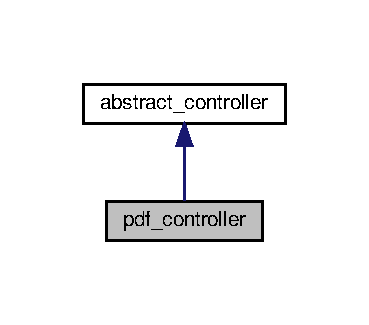
\includegraphics[width=177pt]{classpdf__controller__inherit__graph}
\end{center}
\end{figure}


Collaboration diagram for pdf\+\_\+controller\+:\nopagebreak
\begin{figure}[H]
\begin{center}
\leavevmode
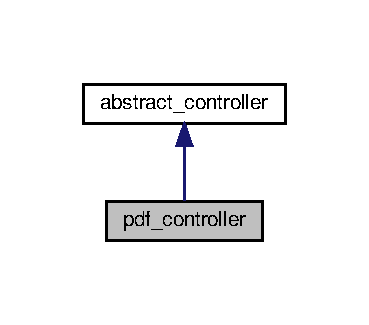
\includegraphics[width=177pt]{classpdf__controller__coll__graph}
\end{center}
\end{figure}
\subsection*{Public Member Functions}
\begin{DoxyCompactItemize}
\item 
\mbox{\Hypertarget{classpdf__controller_a476c4b6bab7a40ea57793806faf334b8}\label{classpdf__controller_a476c4b6bab7a40ea57793806faf334b8}} 
std\+::unordered\+\_\+map$<$ \hyperlink{classcoordinate__phase__space__time}{coordinate\+\_\+phase\+\_\+space\+\_\+time}, double $>$ {\bfseries assembling\+Multi\+Dim} (std\+::vector$<$ std\+::vector$<$ \hyperlink{classparticle}{particle} $>$ $>$ \&particles\+Time, unsigned int equation\+Type)
\item 
\mbox{\Hypertarget{classpdf__controller_a9f1486ae3b861978069f3b1dcfdb0367}\label{classpdf__controller_a9f1486ae3b861978069f3b1dcfdb0367}} 
std\+::vector$<$ std\+::unordered\+\_\+map$<$ \hyperlink{classcoordinate__phase__space__time}{coordinate\+\_\+phase\+\_\+space\+\_\+time}, double $>$ $>$ {\bfseries assembling\+Multi\+Dim\+\_\+parallel} (std\+::vector$<$ std\+::vector$<$ \hyperlink{classparticle}{particle} $>$ $>$ \&particles\+Time, unsigned int equation\+Type)
\item 
\mbox{\Hypertarget{classpdf__controller_add7f5f1aafd15dfc45623059ad845e34}\label{classpdf__controller_add7f5f1aafd15dfc45623059ad845e34}} 
std\+::vector$<$ std\+::vector$<$ std\+::vector$<$ std\+::vector$<$ double $>$ $>$ $>$ $>$ {\bfseries relaxating\+\_\+\+Gauss\+Seidel\+\_\+4D} (std\+::vector$<$ std\+::vector$<$ std\+::vector$<$ std\+::vector$<$ double $>$$>$$>$$>$ pdf, unsigned int number\+Of\+Relaxation\+Steps)
\item 
\mbox{\Hypertarget{classpdf__controller_a0e5c2d07f1bd3bfacd2494942f7975c1}\label{classpdf__controller_a0e5c2d07f1bd3bfacd2494942f7975c1}} 
double {\bfseries calculate\+\_\+wasserstein\+\_\+metric} (std\+::vector$<$ std\+::vector$<$ \hyperlink{classparticle}{particle} $>$$>$ dist1, std\+::vector$<$ std\+::vector$<$ \hyperlink{classparticle}{particle} $>$$>$ dist2)
\item 
\mbox{\Hypertarget{classpdf__controller_a68925f6754a06e4a83cec462959a5875}\label{classpdf__controller_a68925f6754a06e4a83cec462959a5875}} 
double {\bfseries calculate\+\_\+wasserstein\+\_\+metric\+\_\+histogramm} (std\+::vector$<$ std\+::unordered\+\_\+map$<$ \hyperlink{classcoordinate__phase__space__time}{coordinate\+\_\+phase\+\_\+space\+\_\+time}, double $>$$>$ dist1, std\+::vector$<$ std\+::unordered\+\_\+map$<$ \hyperlink{classcoordinate__phase__space__time}{coordinate\+\_\+phase\+\_\+space\+\_\+time}, double $>$$>$ dist2)
\end{DoxyCompactItemize}


The documentation for this class was generated from the following files\+:\begin{DoxyCompactItemize}
\item 
/home/jan/\+Promotion\+\_\+linux\+P\+C/\+Optim\+\_\+\+V\+S\+T\+R\+A\+P/src/controller/pdf\+\_\+controller.\+h\item 
/home/jan/\+Promotion\+\_\+linux\+P\+C/\+Optim\+\_\+\+V\+S\+T\+R\+A\+P/src/controller/pdf\+\_\+controller.\+cpp\end{DoxyCompactItemize}

\hypertarget{classstepdirection__controller}{}\section{stepdirection\+\_\+controller Class Reference}
\label{classstepdirection__controller}\index{stepdirection\+\_\+controller@{stepdirection\+\_\+controller}}


Inheritance diagram for stepdirection\+\_\+controller\+:\nopagebreak
\begin{figure}[H]
\begin{center}
\leavevmode
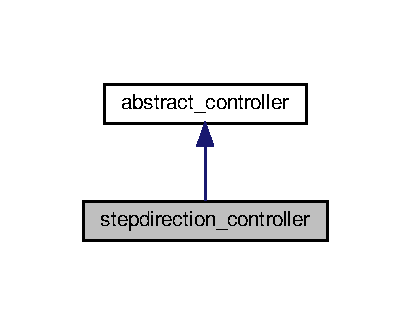
\includegraphics[width=197pt]{classstepdirection__controller__inherit__graph}
\end{center}
\end{figure}


Collaboration diagram for stepdirection\+\_\+controller\+:\nopagebreak
\begin{figure}[H]
\begin{center}
\leavevmode
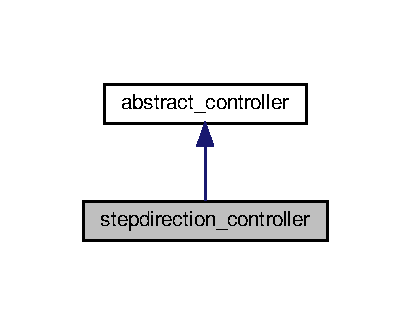
\includegraphics[width=197pt]{classstepdirection__controller__coll__graph}
\end{center}
\end{figure}
\subsection*{Public Member Functions}
\begin{DoxyCompactItemize}
\item 
\mbox{\Hypertarget{classstepdirection__controller_afd3bc683ac79057254e6c61d1cfb4c7d}\label{classstepdirection__controller_afd3bc683ac79057254e6c61d1cfb4c7d}} 
{\bfseries stepdirection\+\_\+controller} (const char $\ast$filename)
\item 
\mbox{\Hypertarget{classstepdirection__controller_ab2d76b39009f8d6c0121288d79c42a9d}\label{classstepdirection__controller_ab2d76b39009f8d6c0121288d79c42a9d}} 
arma\+::mat {\bfseries get\+\_\+stepdirection} (arma\+::mat gradient, arma\+::mat gradient\+\_\+old, arma\+::mat stepdirection\+Old, unsigned int optimization\+\_\+iteration)
\item 
\mbox{\Hypertarget{classstepdirection__controller_a1acb1237378c492ef44a46f8e5fbfce1}\label{classstepdirection__controller_a1acb1237378c492ef44a46f8e5fbfce1}} 
arma\+::mat {\bfseries fixed\+\_\+gradient\+\_\+descent} (arma\+::mat gradient, unsigned int optimization\+\_\+iteration)
\item 
\mbox{\Hypertarget{classstepdirection__controller_ae98ce04e7e3f100d1572992ab43da38a}\label{classstepdirection__controller_ae98ce04e7e3f100d1572992ab43da38a}} 
arma\+::mat {\bfseries ncg\+\_\+scheme\+\_\+\+FR} (arma\+::mat gradient, arma\+::mat gradient\+\_\+old, arma\+::mat stepdirection\+Old, unsigned int optimization\+\_\+iteration)
\item 
\mbox{\Hypertarget{classstepdirection__controller_a63b024e1780f92773e7206f69177af23}\label{classstepdirection__controller_a63b024e1780f92773e7206f69177af23}} 
arma\+::mat {\bfseries ncg\+\_\+scheme\+\_\+\+PR} (arma\+::mat gradient, arma\+::mat gradient\+\_\+old, arma\+::mat stepdirection\+Old, unsigned int optimization\+\_\+iteration)
\item 
\mbox{\Hypertarget{classstepdirection__controller_a86875462174e50ae056d7a1fa10ae41b}\label{classstepdirection__controller_a86875462174e50ae056d7a1fa10ae41b}} 
arma\+::mat {\bfseries ncg\+\_\+scheme\+\_\+\+HZ} (arma\+::mat gradient, arma\+::mat gradient\+\_\+old, arma\+::mat stepdirection\+Old, unsigned int optimization\+\_\+iteration)
\end{DoxyCompactItemize}


The documentation for this class was generated from the following files\+:\begin{DoxyCompactItemize}
\item 
/home/jan/\+Promotion\+\_\+linux\+P\+C/\+Optim\+\_\+\+V\+S\+T\+R\+A\+P/src/optimization/stepdirection\+\_\+controller.\+h\item 
/home/jan/\+Promotion\+\_\+linux\+P\+C/\+Optim\+\_\+\+V\+S\+T\+R\+A\+P/src/optimization/stepdirection\+\_\+controller.\+cpp\end{DoxyCompactItemize}

\hypertarget{classstepsize__controller}{}\section{stepsize\+\_\+controller Class Reference}
\label{classstepsize__controller}\index{stepsize\+\_\+controller@{stepsize\+\_\+controller}}


Inheritance diagram for stepsize\+\_\+controller\+:\nopagebreak
\begin{figure}[H]
\begin{center}
\leavevmode
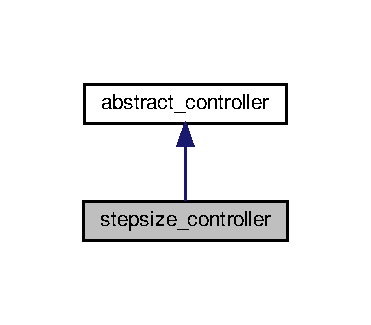
\includegraphics[width=178pt]{classstepsize__controller__inherit__graph}
\end{center}
\end{figure}


Collaboration diagram for stepsize\+\_\+controller\+:\nopagebreak
\begin{figure}[H]
\begin{center}
\leavevmode
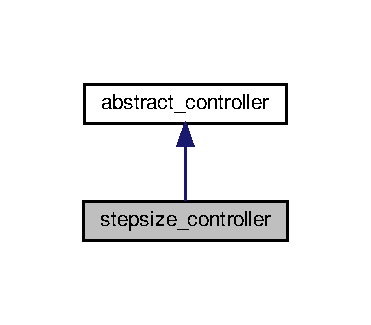
\includegraphics[width=178pt]{classstepsize__controller__coll__graph}
\end{center}
\end{figure}
\subsection*{Public Member Functions}
\begin{DoxyCompactItemize}
\item 
\mbox{\Hypertarget{classstepsize__controller_a40fdd3ec7f99b19f0e7c365dcc839171}\label{classstepsize__controller_a40fdd3ec7f99b19f0e7c365dcc839171}} 
{\bfseries stepsize\+\_\+controller} (const char $\ast$filename)
\item 
\mbox{\Hypertarget{classstepsize__controller_adcdbd7a6b4c5bc02e7d0a9841c5f44c7}\label{classstepsize__controller_adcdbd7a6b4c5bc02e7d0a9841c5f44c7}} 
int {\bfseries calculate\+\_\+stepsize} (arma\+::mat \&gradient, double J0, arma\+::mat \&control, arma\+::mat \&stepdirection, std\+::vector$<$ \hyperlink{classparticle}{particle} $>$ \&input\+Particles, double \&stepsize0)
\end{DoxyCompactItemize}


The documentation for this class was generated from the following files\+:\begin{DoxyCompactItemize}
\item 
/home/jan/\+Promotion\+\_\+linux\+P\+C/\+Optim\+\_\+\+V\+S\+T\+R\+A\+P/src/optimization/stepsize\+\_\+controller.\+h\item 
/home/jan/\+Promotion\+\_\+linux\+P\+C/\+Optim\+\_\+\+V\+S\+T\+R\+A\+P/src/optimization/stepsize\+\_\+controller.\+cpp\end{DoxyCompactItemize}

%--- End generated contents ---

% Index
\backmatter
\newpage
\phantomsection
\clearemptydoublepage
\addcontentsline{toc}{chapter}{Index}
\printindex

\end{document}
